
\subsection{Overview and Scope}
\label{sec:marvin-overview}

This part of the project covers two consecutive processing stages: rigid registration of partially overlapping dental point clouds and surface reconstruction of the resulting merged point cloud. Image acquisition and point-cloud generation are handled by the preceding reconstruction stage; the present contribution starts with multiple point-cloud fragments in different local coordinate systems and ends with an explicit triangular surface model.

The development was deliberately organized as an experimental selection process rather than around a single preselected algorithm. Five pairwise registration methods were first screened on controlled synthetic dental-like data. The most promising approaches were then re-evaluated on five distinct dental model sets comprising ten upper- and lower-jaw STL meshes. Each mesh was sampled into a point cloud, split into overlapping fragments, and displaced by known rigid motions. This broader validation stage changed the final registration decision from Fast Global Registration (FGR) to RANSAC-based global registration. Surface reconstruction was evaluated in the same way: Poisson Surface Reconstruction and the Ball Pivoting Algorithm (BPA) were first compared on the synthetic dataset and then re-evaluated across all ten realistic jaw meshes.

\begin{figure*}[!t]
    \centering
    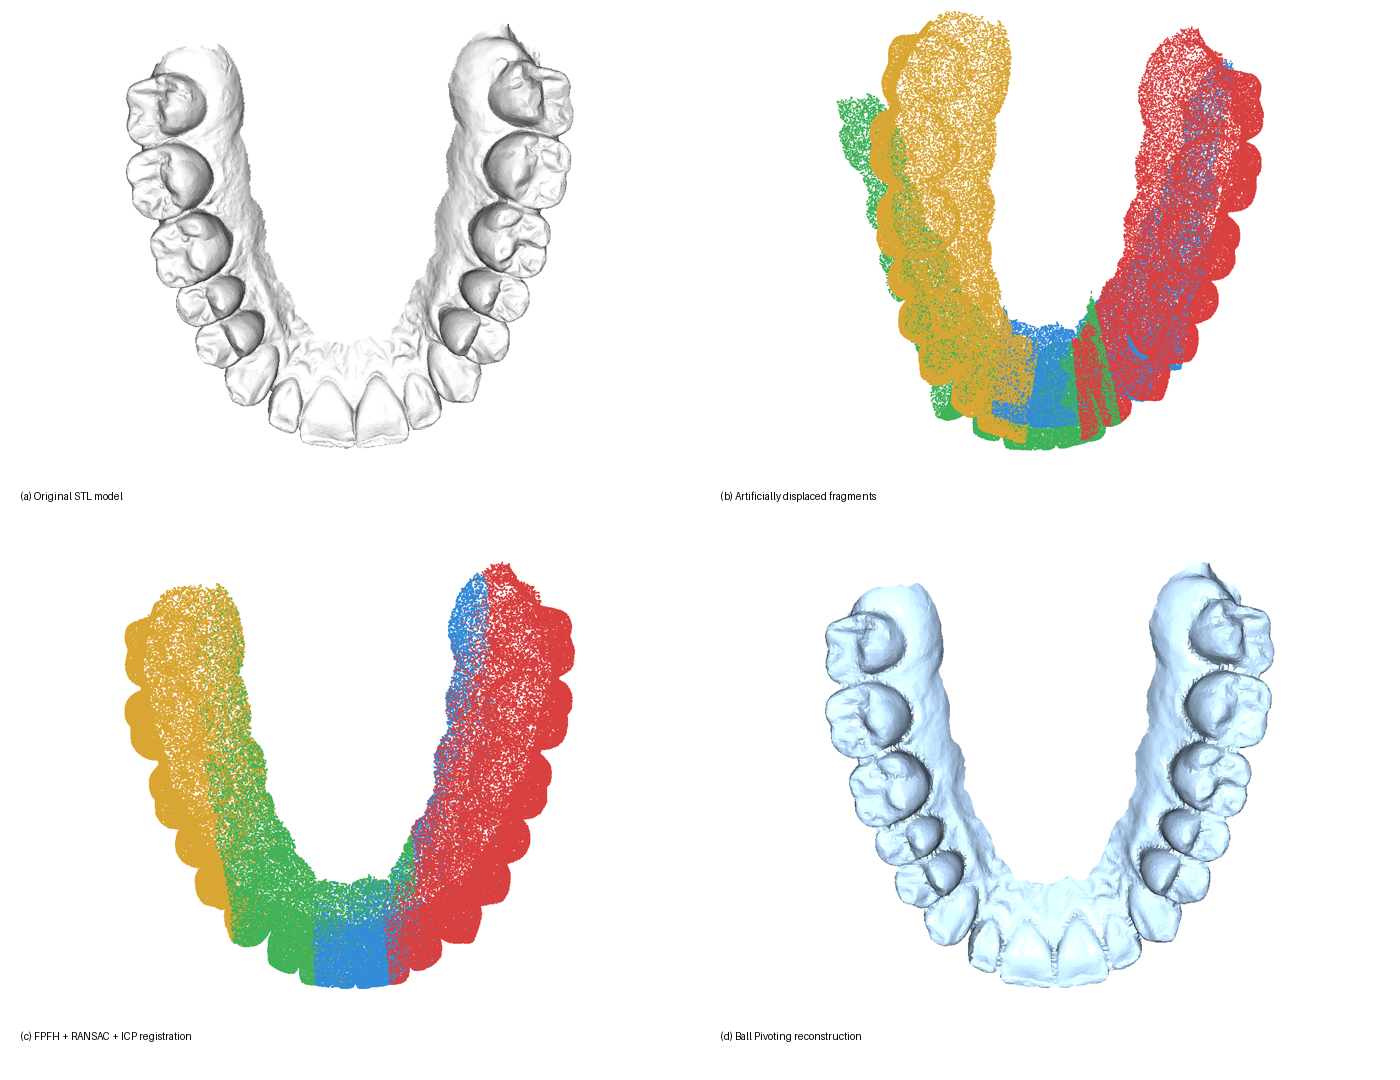
\includegraphics[width=0.96\textwidth]{assets/marvin/realistic_validation_workflow.png}
    \caption{Representative realistic-validation workflow using Model~1 upper jaw. The original STL surface is sampled, split into overlapping fragments, displaced by known rigid transformations, registered with FPFH + RANSAC + Point-to-Plane ICP, and reconstructed with Ball Pivoting. Quantitative evaluation was performed on ten jaw meshes.}
    \label{fig:realistic-validation-workflow}
\end{figure*}

\subsection{Registration Methods}
\label{sec:marvin-registration-methods}

A rigid transformation maps a source point $\mathbf{p}$ to a target point $\mathbf{p}'$ by
\begin{equation}
    \mathbf{p}' = R\mathbf{p} + \mathbf{t},
\end{equation}
where $R\in SO(3)$ is the rotation matrix and $\mathbf{t}\in\mathbb{R}^{3}$ is the translation vector. The implementation consistently uses the convention source $\rightarrow$ target. This convention is especially important when pairwise transformations are chained during multiway registration.

Five registration variants were implemented. Point-to-Point ICP and Point-to-Plane ICP follow the classical local ICP formulation \cite{kraus_besl1992,kraus_chen1992}. Generalized ICP (GICP) extends local matching by incorporating local covariance information \cite{kraus_segal2009}. The two global-to-local pipelines first compute Fast Point Feature Histogram (FPFH) descriptors \cite{kraus_rusu2009}, perform either RANSAC-based feature matching or FGR \cite{kraus_zhou2016}, and then refine the resulting transformation with Point-to-Plane ICP \cite{kraus_lyu2024}.

\begin{table}[!t]
\centering
\footnotesize
\setlength{\tabcolsep}{3pt}
\begin{tabularx}{\columnwidth}{@{}lYY@{}}
\toprule
\textbf{Method} & \textbf{Main advantage} & \textbf{Main limitation} \\
\midrule
Point-to-Point ICP & Simple and fast local refinement & Small capture range \\
Point-to-Plane ICP & Accurate local surface alignment & Requires normals and a good initial pose \\
Generalized ICP & Strong local surface adaptation & Still initialization dependent \\
FPFH + RANSAC + ICP & Large capture range and robust global hypotheses & Stochastic and slower \\
FPFH + FGR + ICP & Fast global initialization with ICP refinement & Sensitive to ambiguous feature correspondences \\
\bottomrule
\end{tabularx}
\caption{Implemented registration methods.}
\label{tab:registration-methods}
\end{table}

All algorithms share the same preprocessing wherever possible. Point clouds are voxel-downsampled with a voxel size of $0.5$, normals are estimated within a radius of $2.0$ voxel sizes using at most 30 neighbors, and FPFH descriptors use a radius of $5.0$ voxel sizes and at most 100 neighbors. RANSAC uses three correspondences per hypothesis, up to 100,000 iterations, and a confidence of $0.999$. The final local refinement uses Point-to-Plane ICP with a correspondence distance of $0.4$ voxel sizes. Open3D 0.19.0 provides the geometric processing and registration primitives \cite{kraus_open3d019}.

\begin{figure}[!t]
\centering
\begin{tikzpicture}[
    node distance=4mm,
    box/.style={draw, rounded corners, align=center, minimum width=0.88\columnwidth, minimum height=6mm, font=\footnotesize},
    arr/.style={-{Latex[length=2mm]}, thick}
]
\node[box] (pre) {Voxel downsampling + normal estimation};
\node[box, below=of pre] (fpfh) {FPFH descriptor computation};
\node[box, below=of fpfh] (ransac) {RANSAC global registration};
\node[box, below=of ransac] (icp) {Point-to-Plane ICP refinement};
\node[box, below=of icp] (eval) {Fitness, RMSE and ground-truth transform error};
\draw[arr] (pre) -- (fpfh);
\draw[arr] (fpfh) -- (ransac);
\draw[arr] (ransac) -- (icp);
\draw[arr] (icp) -- (eval);
\end{tikzpicture}
\caption{Final pairwise registration pipeline after realistic validation.}
\label{fig:final-ransac-pipeline}
\end{figure}

\subsection{Implementation Structure and Evaluation Metrics}
\label{sec:marvin-implementation-metrics}

The implementation uses a small modular Python/Open3D architecture so that preprocessing, algorithms, evaluation, visualization, and mesh construction can be exchanged independently. The registration layer contains the five pairwise methods behind a common result interface, while the reconstruction layer contains Poisson/BPA reconstruction, cleanup, topology analysis, simplification, and export. This separation was important for the experimental workflow because the same preprocessing and evaluation code could be reused for synthetic and realistic datasets.

\begin{table}[!t]
\centering
\footnotesize
\setlength{\tabcolsep}{3pt}
\begin{tabularx}{\columnwidth}{@{}lY@{}}
\toprule
\textbf{Component} & \textbf{Responsibility} \\
\midrule
Preprocessing & Voxel downsampling, normal estimation, FPFH descriptors \\
Registration algorithms & P2P ICP, P2Plane ICP, GICP, FPFH+RANSAC+ICP, FPFH+FGR+ICP \\
Evaluation & Fitness, inlier RMSE, translation/rotation ground-truth error \\
Multiway registration & Pairwise chaining, pose evaluation, merged cloud export \\
Mesh reconstruction & Poisson and Ball Pivoting \\
Mesh analysis & Components, manifold tests, self-intersections, bidirectional distances \\
Mesh export & Simplification, cleanup, PLY/STL serialization and reload test \\
\bottomrule
\end{tabularx}
\caption{Functional structure of the implemented registration and model-construction pipeline.}
\label{tab:software-structure}
\end{table}

\paragraph{Software architecture.}
The code base separates the importable implementation under \texttt{src/registration3d} from experiment drivers, diagnostic scripts, and report-visualization utilities. Within the core package, registration algorithms follow a strategy-style interface: Point-to-Point ICP, Point-to-Plane ICP, GICP, FPFH+RANSAC+ICP, and FPFH+FGR+ICP expose the same \texttt{register(...)} operation and return a standardized result object. This allows the same evaluator and benchmark logic to be reused without algorithm-specific branches. The two feature-based methods additionally share the same FPFH extractor. Multiway registration accepts an interchangeable pairwise registration strategy and produces a merged point cloud, which is deliberately treated as the boundary between registration and surface reconstruction. The mesh stage is similarly separated into reconstruction, cleanup, topology/distance evaluation, simplification, and export.

\begin{samepage}
When ground truth is available, translation error is computed as
\begin{equation}
    e_t = \lVert \mathbf{t}_{est} - \mathbf{t}_{GT} \rVert_2,
\end{equation}
and rotation error as
\begin{equation}
    e_R = \cos^{-1}\left(\frac{\mathrm{tr}(R_{est}R_{GT}^{T})-1}{2}\right).
\end{equation}
\end{samepage}
The realistic robustness study classifies a result as successful when $e_t\leq1$ model unit and $e_R\leq1^\circ$. This explicit transform-based criterion avoids the ambiguity of relying only on fitness or inlier RMSE.

\subsection{Synthetic Registration Evaluation}
\label{sec:marvin-synthetic-registration}

\subsubsection{Evaluation Setup}

Synthetic dental-like source and target clouds were generated with known rigid ground truth. Four disturbance variables were varied independently: overlap, rotation, translation, and additive positional noise. Each condition was evaluated in 10 reproducible repetitions. Within a given stress-test series, the same repetition index uses the same dataset seed across all values of the varied parameter, while stochastic registration methods receive reproducible algorithm seeds. This design reduces unintended variation between neighboring conditions and allows direct evaluation of the estimated transformation rather than relying only on correspondence-based metrics.

\begin{table}[H]
\centering
\footnotesize
\begin{tabularx}{\columnwidth}{@{}lY@{}}
\toprule
\textbf{Experiment} & \textbf{Tested values} \\
\midrule
Overlap & 0.20, 0.30, 0.40, 0.50, 0.60, 0.70, 0.80 \\
Rotation & $0^\circ$, $5^\circ$, $10^\circ$, $20^\circ$, $30^\circ$, $40^\circ$, $60^\circ$ \\
Translation & 0, 1, 2, 4, 6, 8, 12 \\
Noise standard deviation & 0, 0.01, 0.025, 0.05, 0.10, 0.20 \\
\bottomrule
\end{tabularx}
\caption{Controlled synthetic registration experiments. Each parameter value was evaluated with $n=10$ reproducible repetitions.}
\label{tab:synthetic-registration-setup}
\end{table}

The principal metrics were fitness, inlier RMSE, translation error, rotation error, runtime, and success rate. Fitness and inlier RMSE alone were not treated as correctness guarantees: repetitive dental geometry can produce geometrically plausible but semantically incorrect correspondences. Whenever ground truth was available, translation and rotation errors were therefore decisive.

\begin{figure*}[!t]
\centering
\begin{subfigure}[t]{0.48\textwidth}
    \centering
    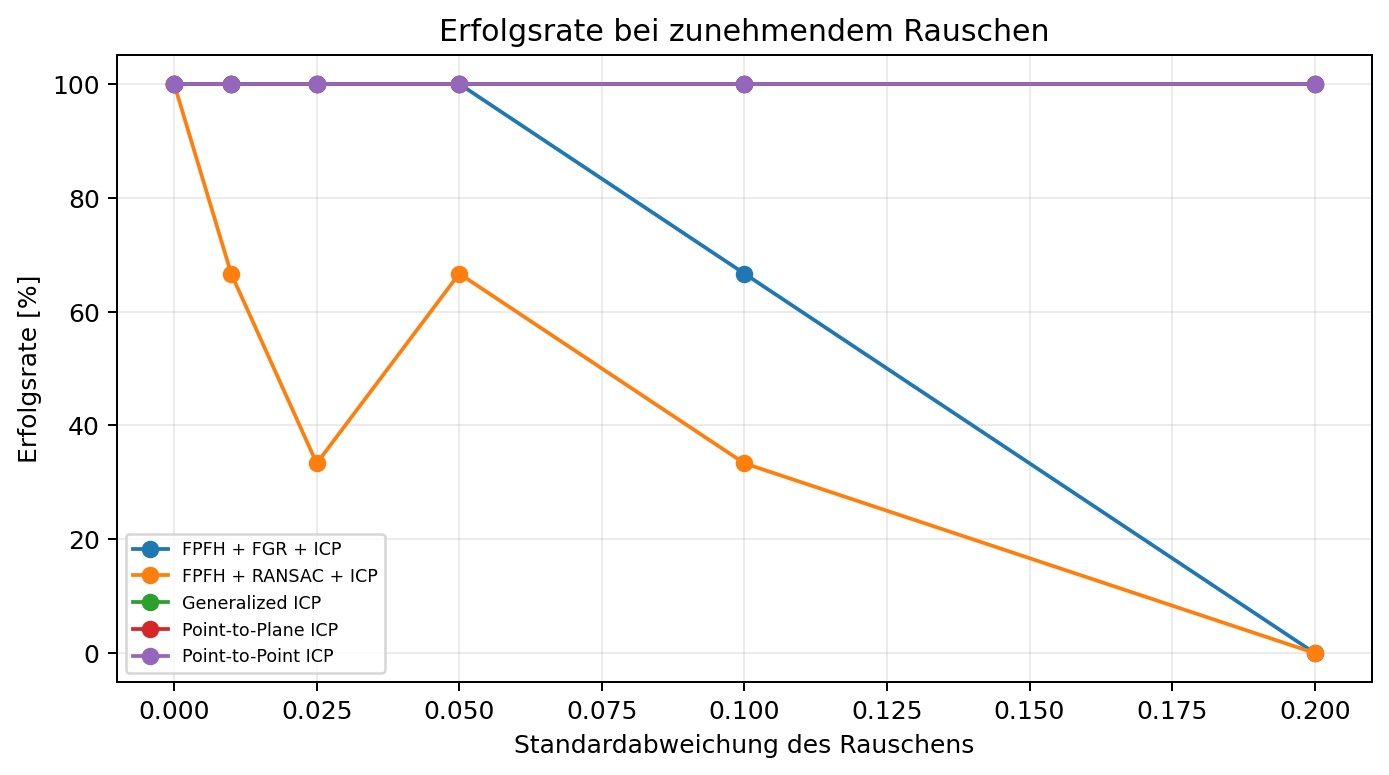
\includegraphics[width=\linewidth]{assets/marvin/noise_success_rate.png}
    \caption{Noise.}
\end{subfigure}
\hfill
\begin{subfigure}[t]{0.48\textwidth}
    \centering
    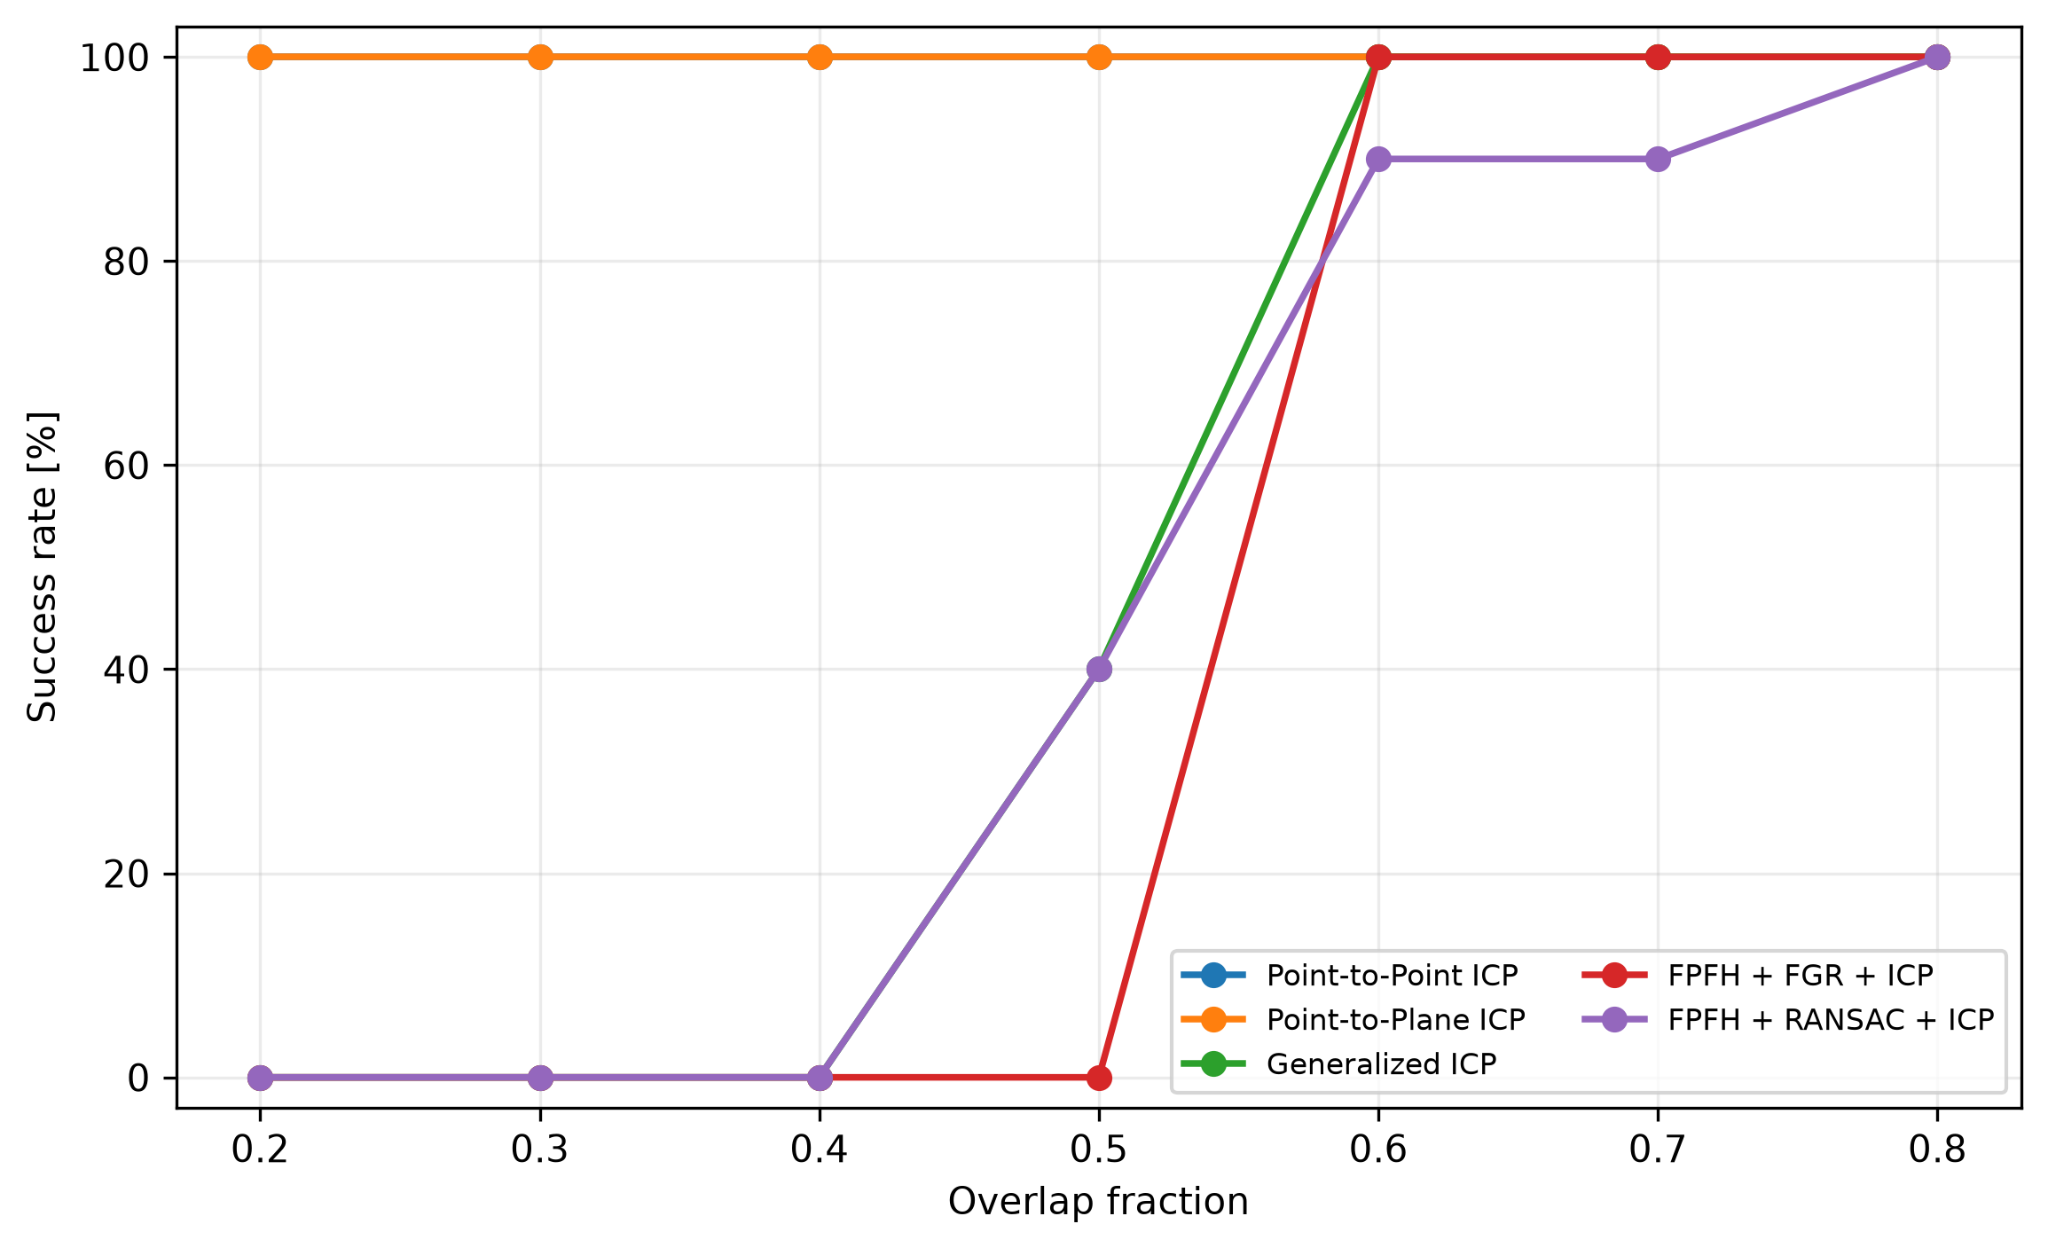
\includegraphics[width=\linewidth]{assets/marvin/overlap_success_rate.png}
    \caption{Overlap.}
\end{subfigure}

\vspace{2mm}

\begin{subfigure}[t]{0.48\textwidth}
    \centering
    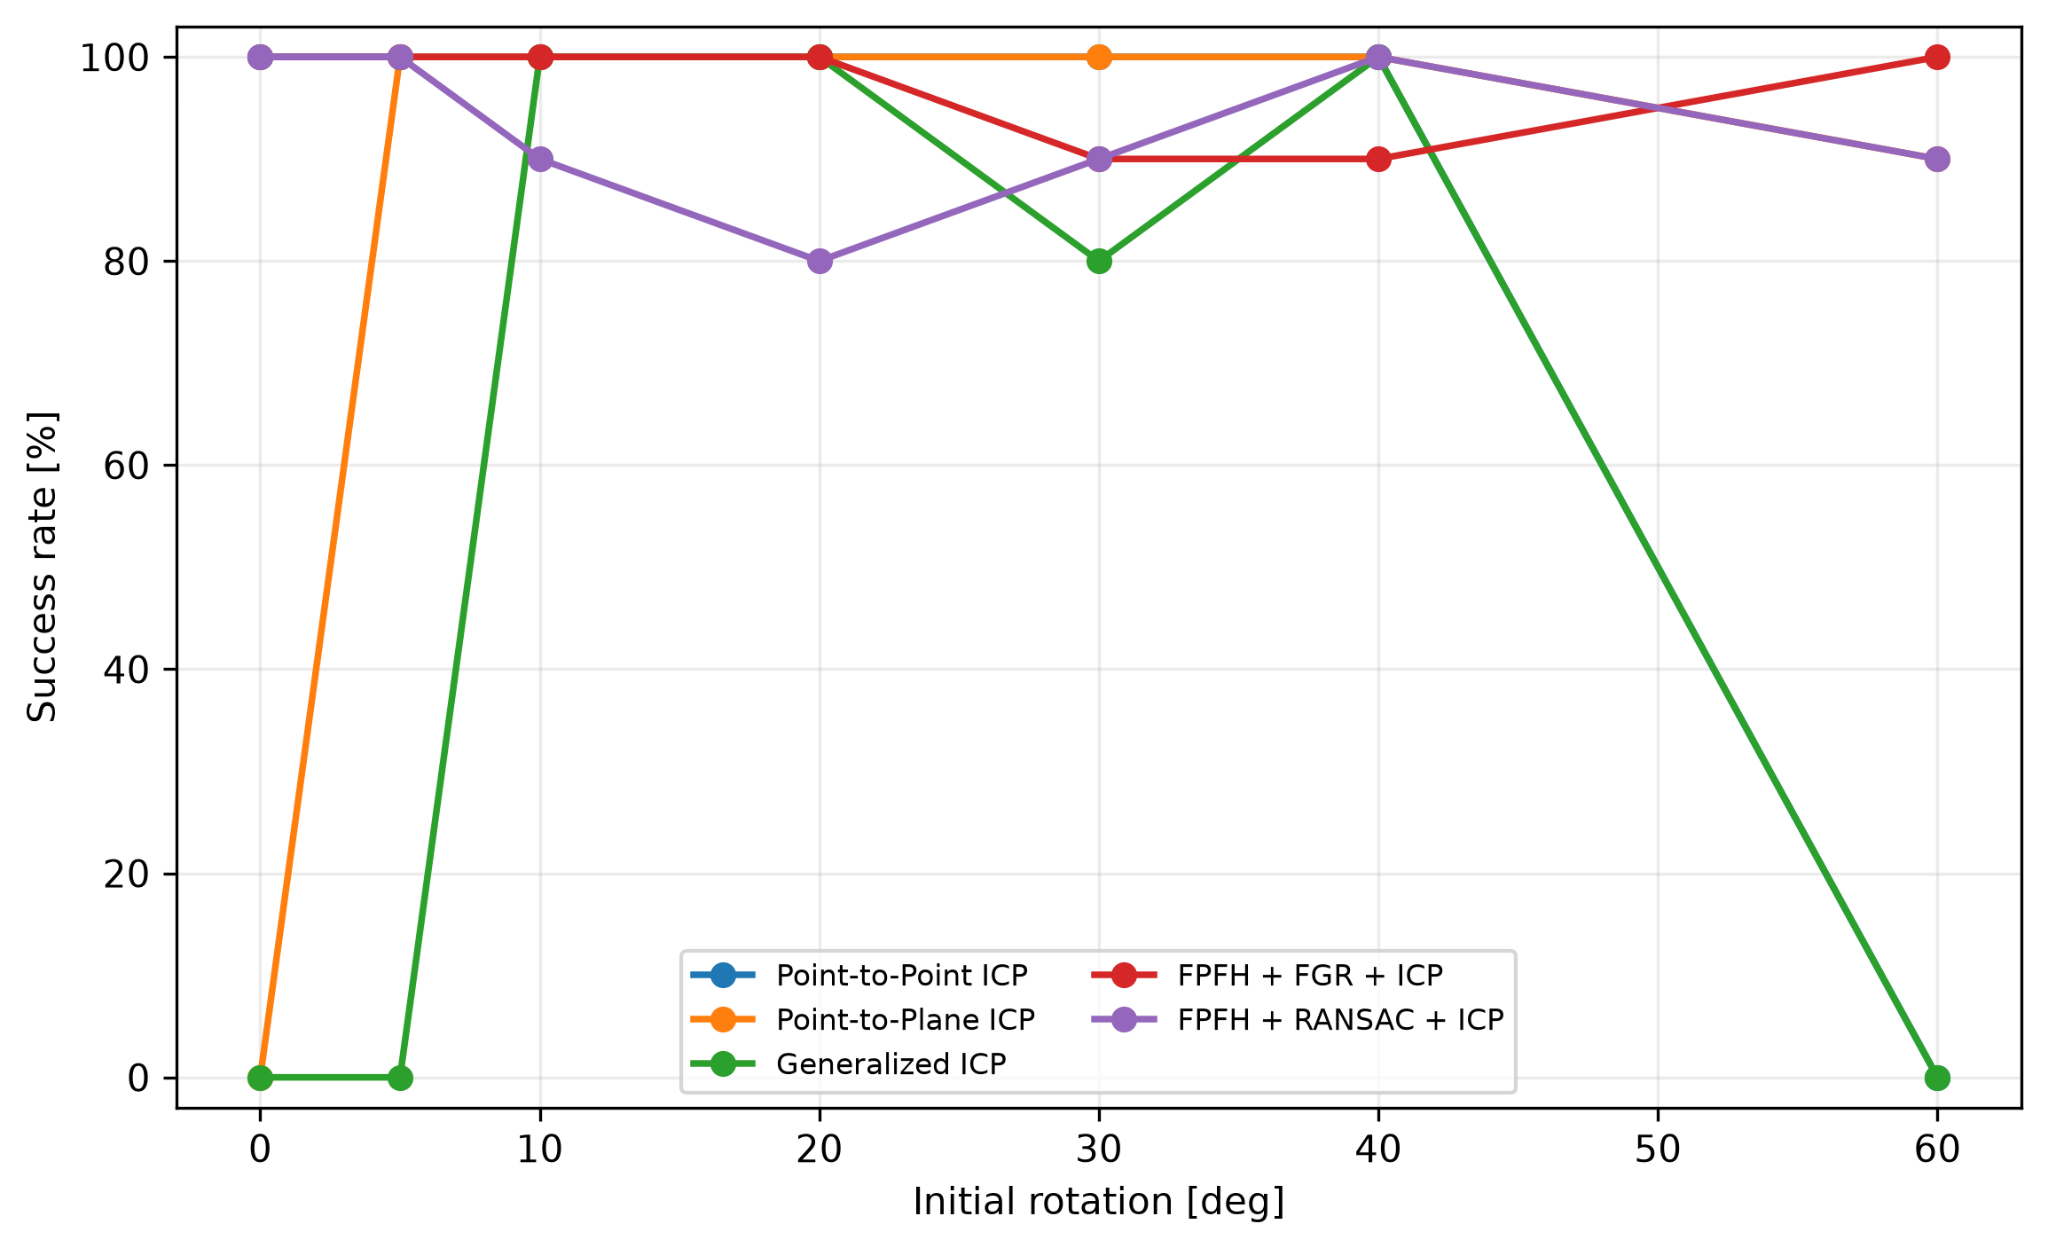
\includegraphics[width=\linewidth]{assets/marvin/rotation_success_rate.png}
    \caption{Rotation.}
\end{subfigure}
\hfill
\begin{subfigure}[t]{0.48\textwidth}
    \centering
    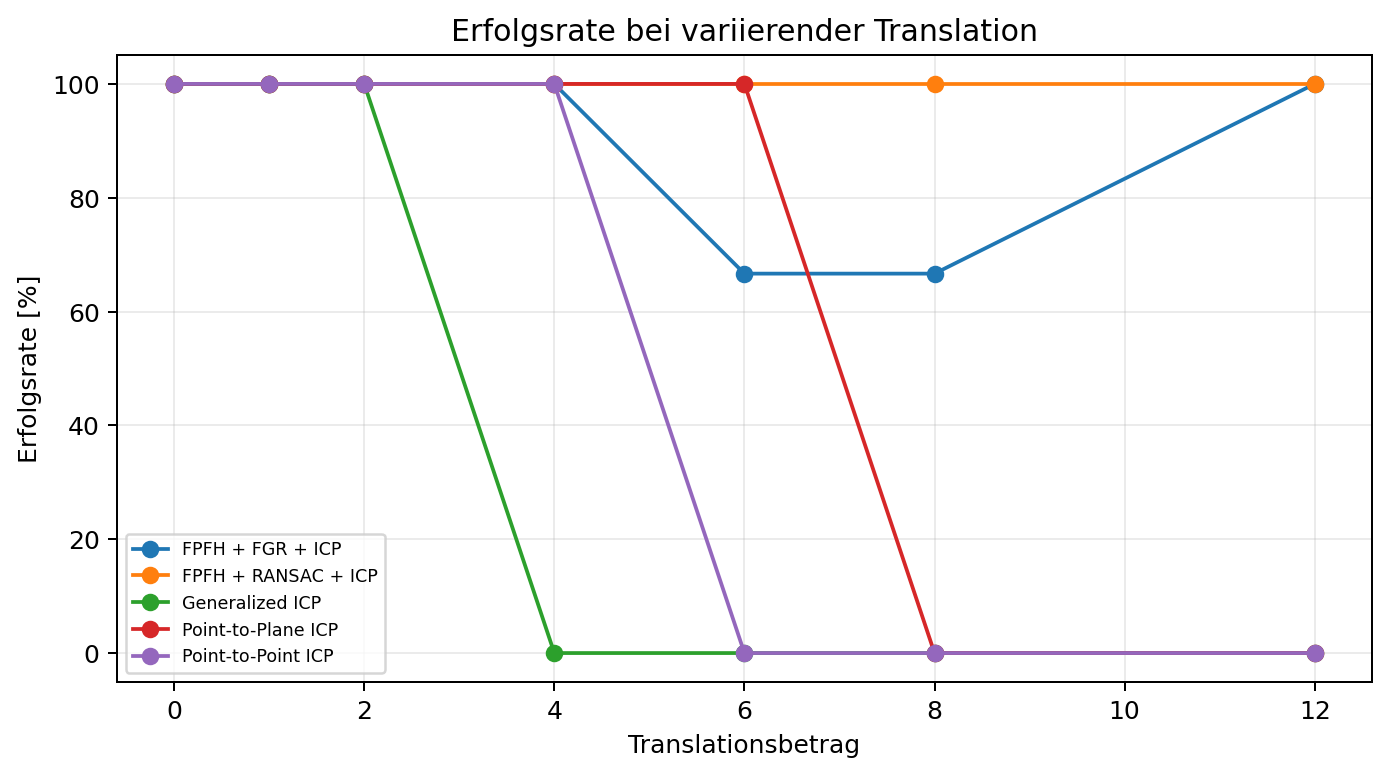
\includegraphics[width=\linewidth]{assets/marvin/translation_success_rate.png}
    \caption{Translation.}
\end{subfigure}
\caption{Success-rate curves from the controlled synthetic pairwise experiments ($n=10$ repetitions per parameter value). The curves should be interpreted as empirical behavior on the specific dental-like geometry rather than as universal monotonic capture-range characteristics.}
\label{fig:synthetic-success-rates}
\end{figure*}

\begin{table*}[!t]
\centering
\footnotesize
\setlength{\tabcolsep}{4pt}
\begin{tabularx}{\textwidth}{@{}lYYYYY@{}}
\toprule
\textbf{Stress case} & \textbf{P2P ICP} & \textbf{P2Plane ICP} & \textbf{GICP} & \textbf{RANSAC + ICP} & \textbf{FGR + ICP} \\
\midrule
Favorable initialization & Very strong & Very strong & Very strong & Strong & Strong \\
Large translation & Capture-range failures & Capture-range failures & Capture-range failures & Robust global recovery & Robust global recovery \\
Low overlap & Can converge locally if initialized well & Can converge locally if initialized well & Can remain locally accurate & Ambiguous feature matches & Ambiguous feature matches \\
High rotation & Fails at the largest tested angle & Non-monotonic local-minimum behavior & Strongly non-monotonic & Large capture range & Large capture range \\
Strong synthetic noise & Stable only with favorable initialization & Stable only with favorable initialization & Stable only with favorable initialization & Global feature matching degraded & Global feature matching degraded \\
\bottomrule
\end{tabularx}
\caption{Qualitative behavior observed in the controlled synthetic stress tests. The table summarizes failure modes rather than claiming a universal algorithm ranking.}
\label{tab:synthetic-behavior-summary}
\end{table*}

\paragraph{Interpretation of overlap and rotation.}
The updated 10-repeat overlap study removes an apparent non-monotonicity that was present in an earlier exploratory plot. For FPFH + RANSAC + ICP, the observed success rates increase from 0\% at overlaps 0.20--0.40 to 40\% at 0.50, 90\% at 0.60 and 0.70, and 100\% at 0.80. FGR shows an even sharper transition, remaining at 0\% through 0.50 and reaching 100\% from 0.60 onward. This supports the interpretation that, on the synthetic dental-like geometry, the feature-based methods require a sufficiently large common visible region before FPFH correspondences become reliably distinctive.

The rotation series exhibits a notable non-monotonic behavior for Point-to-Plane ICP. An input rotation of $0^\circ$ does not correspond to a perfectly aligned pair: the series keeps overlap at 0.60, translation magnitude at 3 model units, and Gaussian noise at $\sigma=0.02$. Under this translation-only displacement, Point-to-Plane ICP converged consistently to an incorrect local solution, with mean translation error 3.5399 model units and mean rotation error $7.336^\circ$. For rotations from $5^\circ$ through $40^\circ$, the altered correspondence configuration instead led to a favorable convergence basin, producing 100\% success and mean translation errors of approximately 0.017--0.021 model units. At $60^\circ$, one of ten runs failed, reducing success to 90\%. This result is interpreted as a dataset-specific local-minimum effect: it does not imply that adding rotation generally improves ICP, but rather that the correspondence landscape of the repetitive synthetic geometry changes with the applied pose.


GICP shows a similarly non-monotonic rotation response, although for a slightly different reason. It is still a local iterative method and therefore remains sensitive to the nearest-neighbor correspondences induced by the initial pose. In addition, its residual is weighted by local covariance information, so a change in relative orientation alters both the correspondences and the covariance-weighted objective. On the repetitive synthetic dental-like geometry, different input rotations can therefore move the optimizer between substantially different convergence basins. The observed fluctuations are interpreted as correspondence and local-minimum effects of this particular dataset, not as a monotonic relationship between larger rotations and better or worse GICP performance.

\subsubsection{Synthetic Findings and Provisional Selection}

The synthetic experiments highlighted the expected trade-off. Local ICP variants were fast and highly accurate whenever the initial alignment remained inside their capture range, but they failed for larger displacements. Feature-based global registration handled larger initial pose differences but was more sensitive to low overlap, repetitive geometry, and noise.

Under the original synthetic benchmark, FPFH + FGR + Point-to-Plane ICP provided the most attractive overall compromise between global capture range, precision after local refinement, and runtime. It was therefore selected \emph{provisionally} for the first multiway baseline. This was not treated as a universal ranking; the later realistic validation was explicitly intended to challenge this choice.

A four-fragment synthetic multiway test confirmed that FGR + ICP could produce a precise chain under the controlled test conditions. The maximum node translation error was approximately $0.0047$ and the maximum rotation error approximately $0.035^\circ$, while the merged cloud contained 22,022 points. Additional multi-start and cycle-consistency experiments showed, however, that high fitness can still occur for incorrect dental alignments. This observation motivated the second validation stage on realistic jaw geometry.

\subsubsection{Synthetic Multiway Baseline and Robustness Analysis}

The synthetic multiway dataset contains four partially overlapping fragments with 13,793, 15,302, 16,193, and 15,069 points. The controlled acquisition model again follows $\mathbf{x}_i=A_i\mathbf{x}_{world}$, so the exact pose of fragment $i$ in the global reference frame is $A_i^{-1}$. For the provisional FGR baseline, only sequential odometry edges were used. Loop closures were deliberately disabled to measure the selected pairwise method without global correction.

\begin{figure}[!t]
\centering
\begin{tikzpicture}[
  node distance=12mm,
  frag/.style={circle,draw,minimum size=8mm,font=\footnotesize},
  odo/.style={-{Latex[length=2mm]},thick},
  loop/.style={-{Latex[length=2mm]},dashed}
]
\node[frag] (f0) {0};
\node[frag, right=of f0] (f1) {1};
\node[frag, right=of f1] (f2) {2};
\node[frag, right=of f2] (f3) {3};
\draw[odo] (f0) -- node[above,font=\scriptsize]{odometry} (f1);
\draw[odo] (f1) -- (f2);
\draw[odo] (f2) -- (f3);
\draw[loop,bend left=35] (f0) to node[above,font=\scriptsize]{candidate loop} (f2);
\draw[loop,bend left=35] (f1) to node[above,font=\scriptsize]{candidate loop} (f3);
\end{tikzpicture}
\caption{Synthetic four-fragment pose-graph concept. Solid edges form the evaluated sequential baseline; dashed loop candidates were examined only in the optional robustness analysis.}
\label{fig:synthetic-pose-graph}
\end{figure}

\begin{table}[H]
\centering
\footnotesize
\begin{tabular}{lrr}
\toprule
\textbf{Odometry edge} & \textbf{Fitness} & \textbf{Inlier RMSE} \\
\midrule
$0\rightarrow1$ & 0.7397 & 0.2499 \\
$1\rightarrow2$ & 0.6904 & 0.2493 \\
$2\rightarrow3$ & 0.6676 & 0.2466 \\
\bottomrule
\end{tabular}
\caption{Synthetic four-fragment FGR + ICP multiway baseline.}
\label{tab:synthetic-multiway-edges}
\end{table}

The resulting pose errors were 0 for fragment 0, 0.00424 / $0.00636^\circ$ for fragment 1, 0.00468 / $0.03513^\circ$ for fragment 2, and 0.00268 / $0.02626^\circ$ for fragment 3. The merged point cloud contained 22,022 points. Thus, under controlled synthetic conditions, sequential accumulation remained small.

A separate robustness analysis generated 20 FGR and 20 RANSAC hypotheses with deterministic seeds, clustered similar transformations, and ranked clusters by median RMSE. Candidate loop closures were also checked for cycle consistency. This procedure could recover correct odometry in ambiguous synthetic cases, but it was intentionally kept separate from the baseline algorithm comparison: cycle consistency can reject some inconsistent hypotheses, yet it cannot prove that a globally self-consistent chain is geometrically correct. The realistic validation therefore remained necessary.

\subsection{Validation on Realistic Dental Geometry}
\label{sec:marvin-realistic-registration}

\subsubsection{Five-Model Dataset Construction}

The realistic validation was expanded to five distinct dental model sets, each containing an upper- and lower-jaw STL mesh. The ten meshes have bounding-box diagonals between 79.696 and 92.084 model units; the ratio between the largest and smallest diagonal is only 1.155, so the same registration parameters can be used without rescaling. Every jaw surface was uniformly sampled to 120,000 points and split into four partially overlapping fragments along the first PCA axis with a nominal overlap of 60\%.

Known rigid acquisition transformations were applied using
\begin{equation}
    \mathbf{x}_i = A_i \mathbf{x}_{\mathrm{world}},
\end{equation}
so that the exact pairwise ground-truth transformation is
\begin{equation}
    T_{i\rightarrow j}^{GT} = A_j A_i^{-1}.
\end{equation}
The STL format itself does not encode physical units. All distances are therefore reported in model units.

\begin{table}[H]
\centering
\footnotesize
\begin{tabularx}{\columnwidth}{@{}lY@{}}
\toprule
\textbf{Property} & \textbf{Five-model validation suite} \\
\midrule
Dental model sets & 5 \\
Jaw meshes & 10 (5 upper, 5 lower) \\
Surface samples per jaw & 120,000 \\
Fragments per jaw & 4 \\
Adjacent pairwise cases & 30 \\
Nominal fragment overlap & 60\% \\
Bounding-box diagonal range & 79.696--92.084 model units \\
\bottomrule
\end{tabularx}
\caption{Realistic five-model validation dataset.}
\label{tab:realistic-dataset}
\end{table}


\begin{figure*}[!t]
\centering
\begin{tikzpicture}[
    node distance=5mm and 7mm,
    box/.style={draw,rounded corners,align=center,minimum width=27mm,minimum height=11mm,font=\footnotesize},
    arr/.style={-{Latex[length=2mm]},thick}
]
\node[box] (stl) {5 dental model sets\\10 jaw STL meshes};
\node[box, right=of stl] (sample) {120,000 sampled\\surface points per jaw};
\node[box, right=of sample] (frag) {4 overlapping fragments\\per jaw};
\node[box, right=of frag] (pairs) {30 adjacent\\pairwise cases};
\node[box, below=of pairs] (pairbench) {5 algorithms\\150 zero-noise runs};
\node[box, left=of pairbench] (noise) {Noise study\\2,400 registrations};
\node[box, left=of noise] (multi) {RANSAC multiway\\10 four-fragment jaws};
\node[box, left=of multi] (mesh) {Surface validation\\40 BPA parameter meshes\\+ 10 Poisson meshes};
\draw[arr] (stl) -- (sample);
\draw[arr] (sample) -- (frag);
\draw[arr] (frag) -- (pairs);
\draw[arr] (pairs) -- (pairbench);
\draw[arr] (pairbench) -- (noise);
\draw[arr] (noise) -- (multi);
\draw[arr] (multi) -- (mesh);
\end{tikzpicture}
\caption{Five-model evaluation protocol. The same ten jaw geometries are propagated from controlled virtual fragmentation through pairwise comparison, noise robustness, sequential multiway registration, and surface-reconstruction validation.}
\label{fig:model-suite-protocol}
\end{figure*}

The experimental protocol deliberately separates geometric diversity from stochastic repetition. The zero-noise benchmark contains 30 distinct adjacent fragment pairs, while the nonzero-noise conditions repeat these same base pairs with three independently seeded perturbations. This distinction prevents repeated perturbations from being presented as additional independent dental geometries. The same fragmented jaws are then reused for the RANSAC multiway experiment and for surface reconstruction, so registration and mesh quality can be evaluated along one consistent end-to-end path.


\begin{figure}[!t]
    \centering
    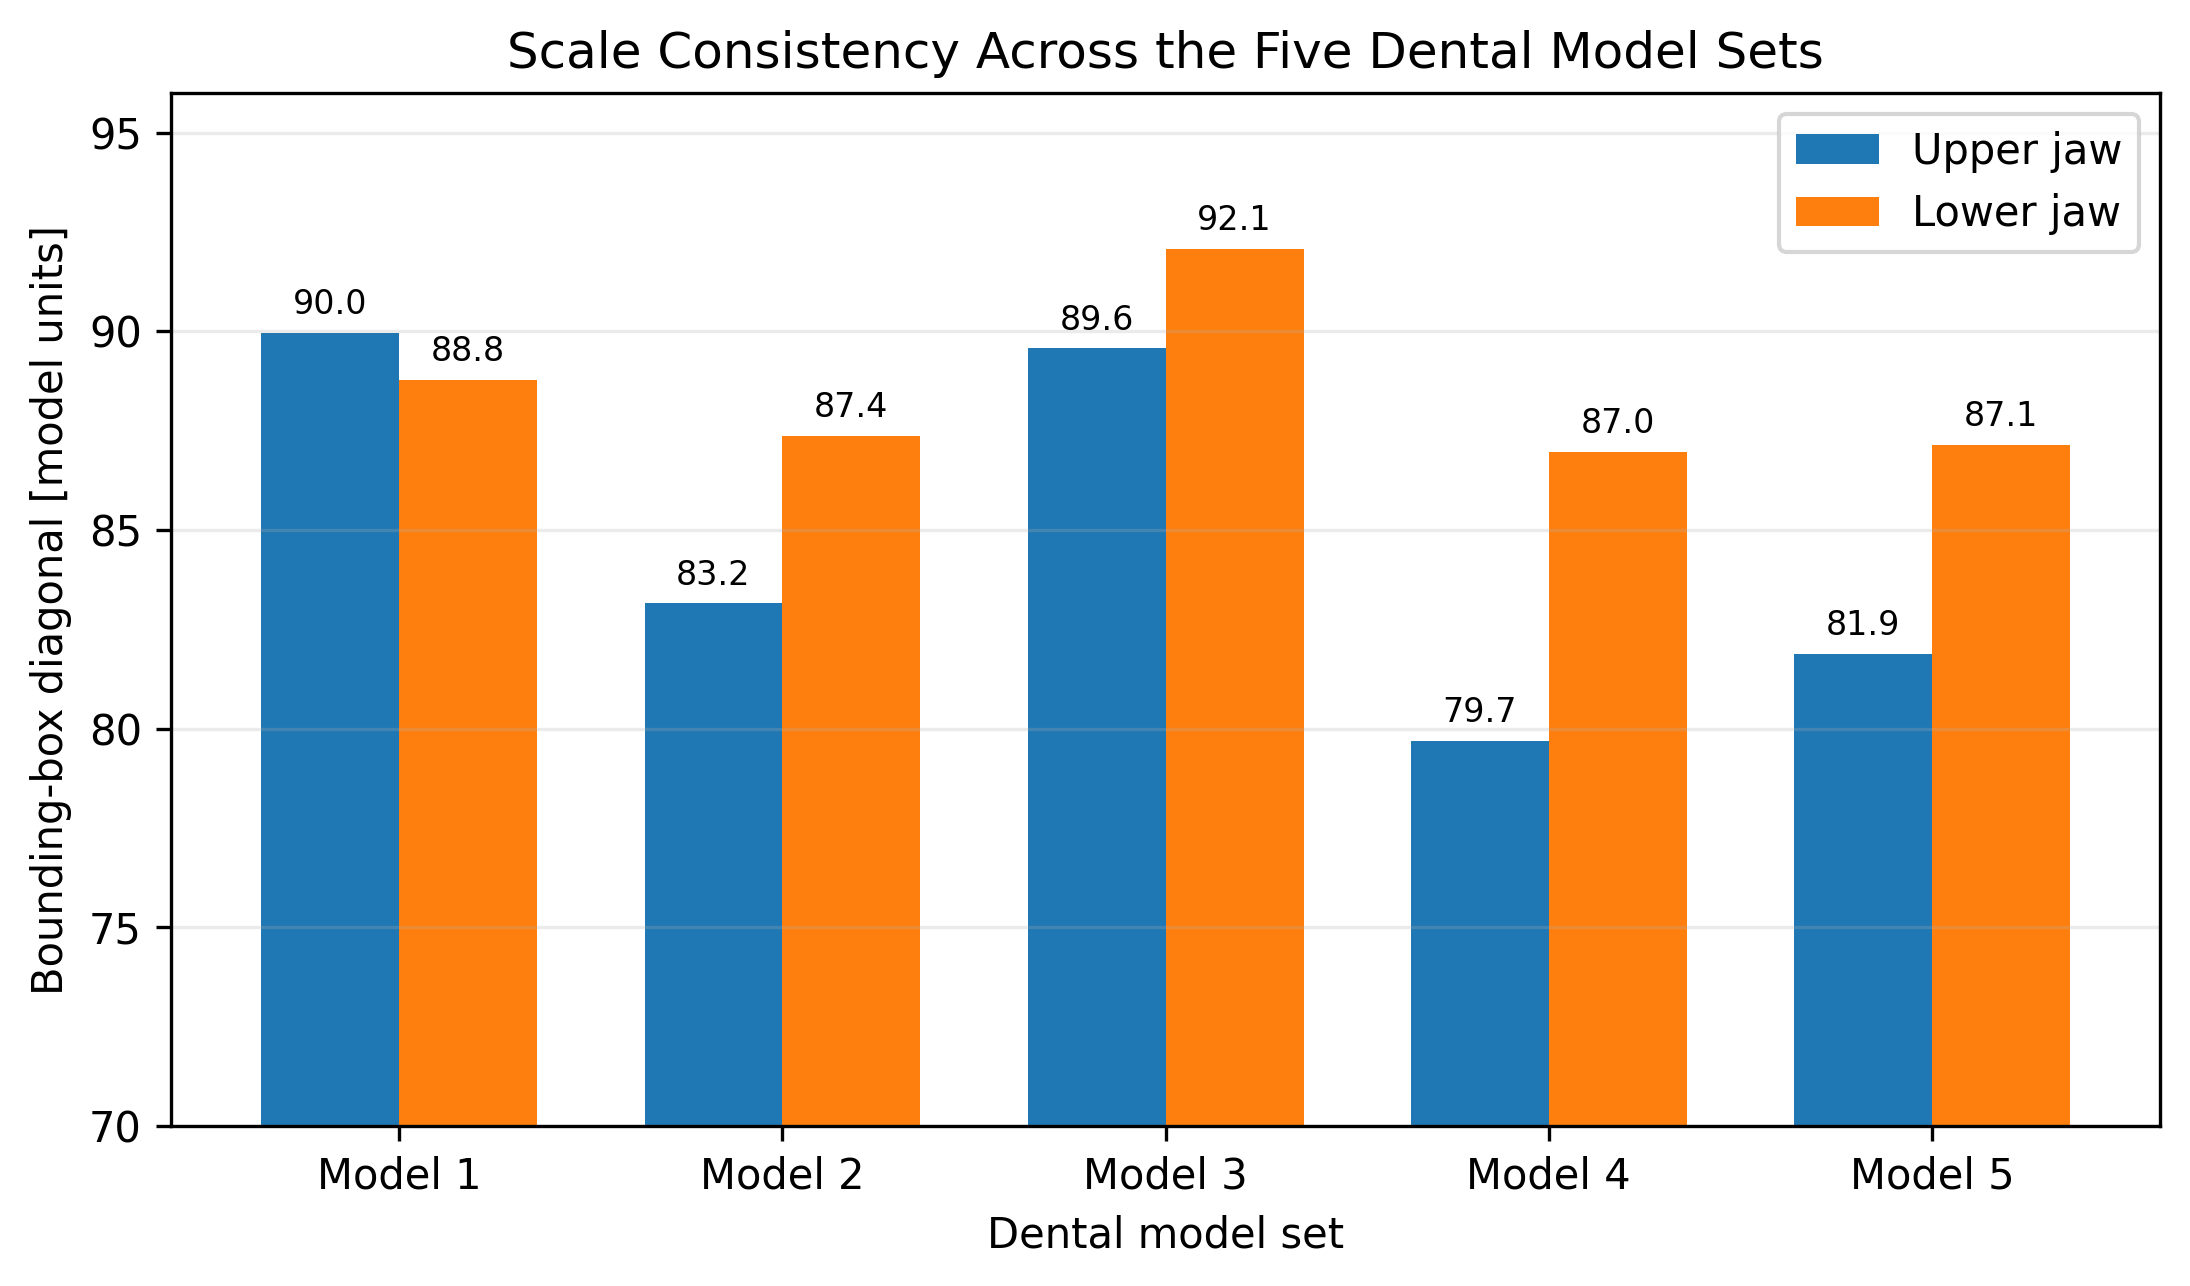
\includegraphics[width=\columnwidth]{assets/marvin/model_suite/model_suite_scale_distribution.png}
    \caption{Bounding-box diagonal for all ten realistic jaw meshes. The relatively narrow range (79.696--92.084 model units) supports using one common registration parameterization, while also showing that the validation does not intentionally span extreme anatomical scale differences.}
    \label{fig:model-suite-scale}
\end{figure}

\begin{figure*}[!t]
\centering
\begin{subfigure}[t]{0.32\textwidth}
    \centering
    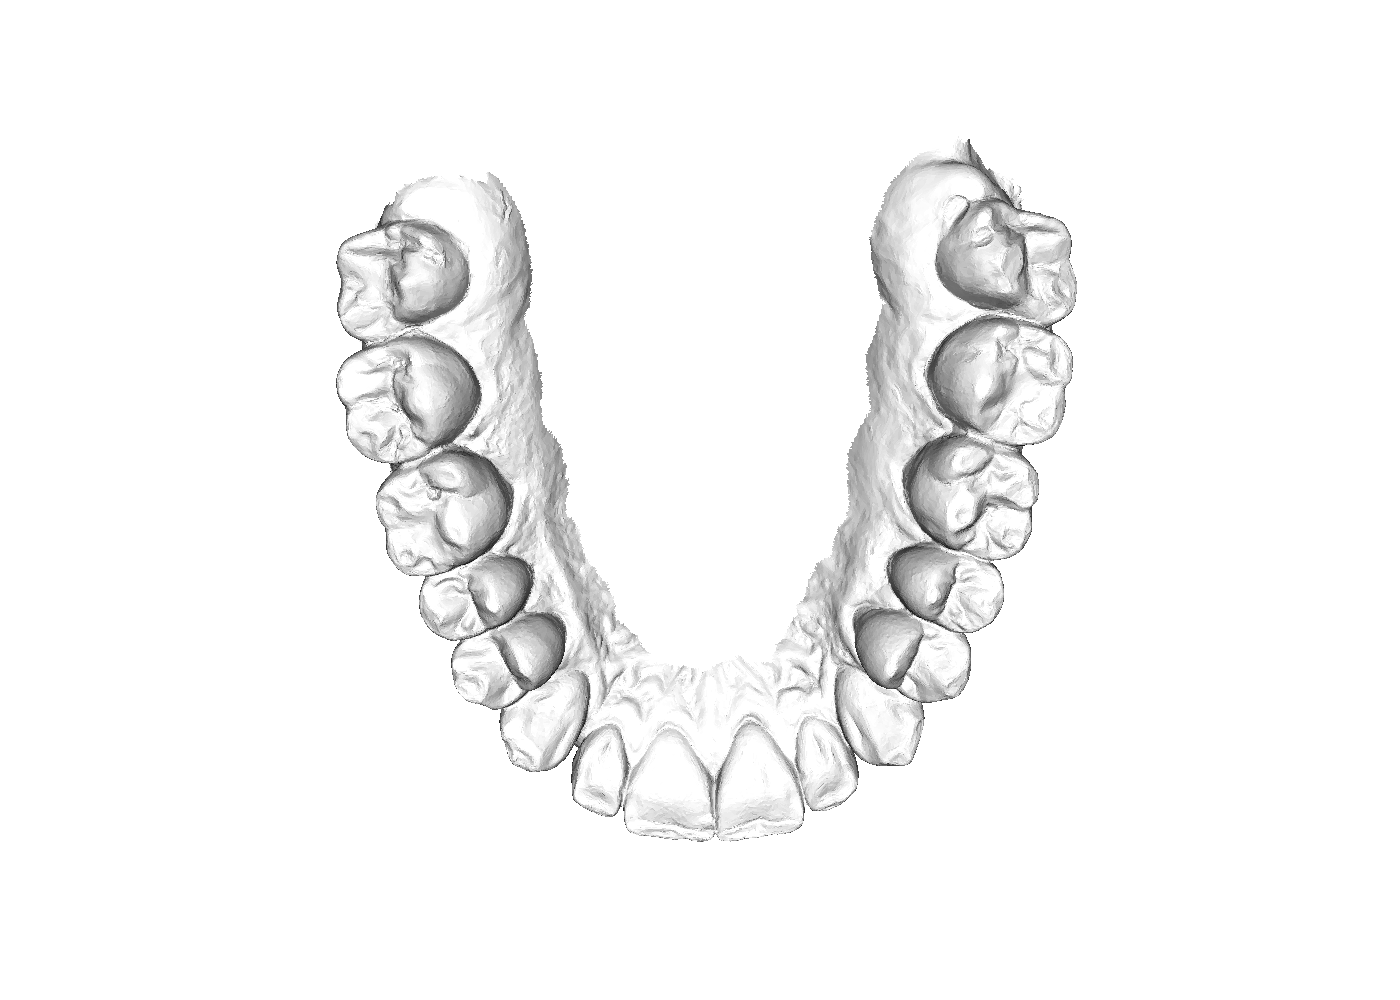
\includegraphics[width=\linewidth]{assets/marvin/upper_original.png}
    \caption{Model~1 upper-jaw STL.}
\end{subfigure}\hfill
\begin{subfigure}[t]{0.32\textwidth}
    \centering
    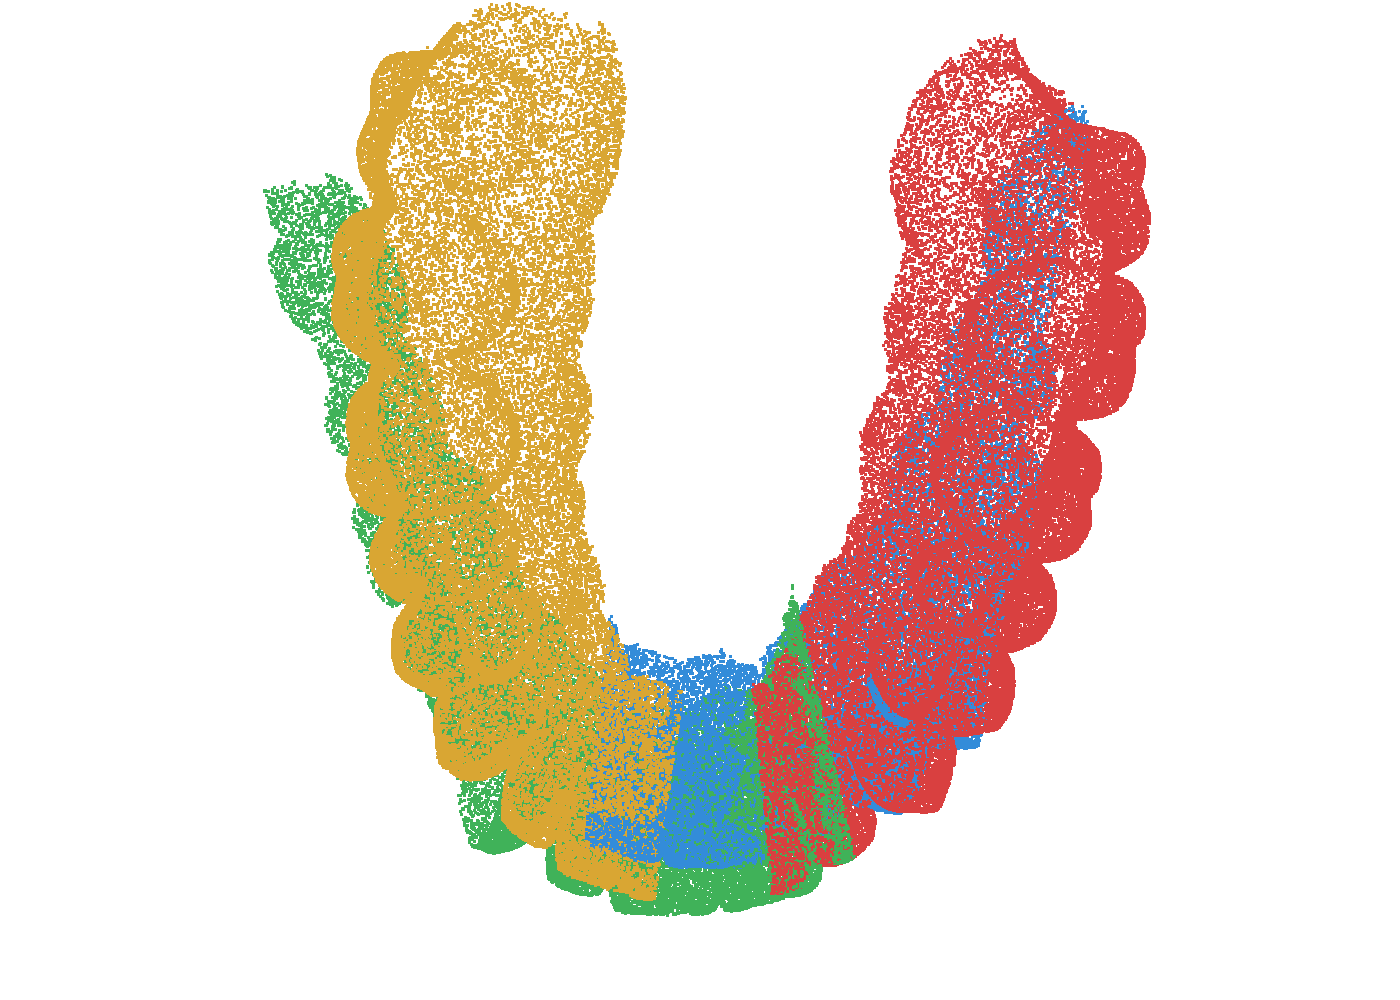
\includegraphics[width=\linewidth]{assets/marvin/upper_displaced.png}
    \caption{Displaced fragments.}
\end{subfigure}\hfill
\begin{subfigure}[t]{0.32\textwidth}
    \centering
    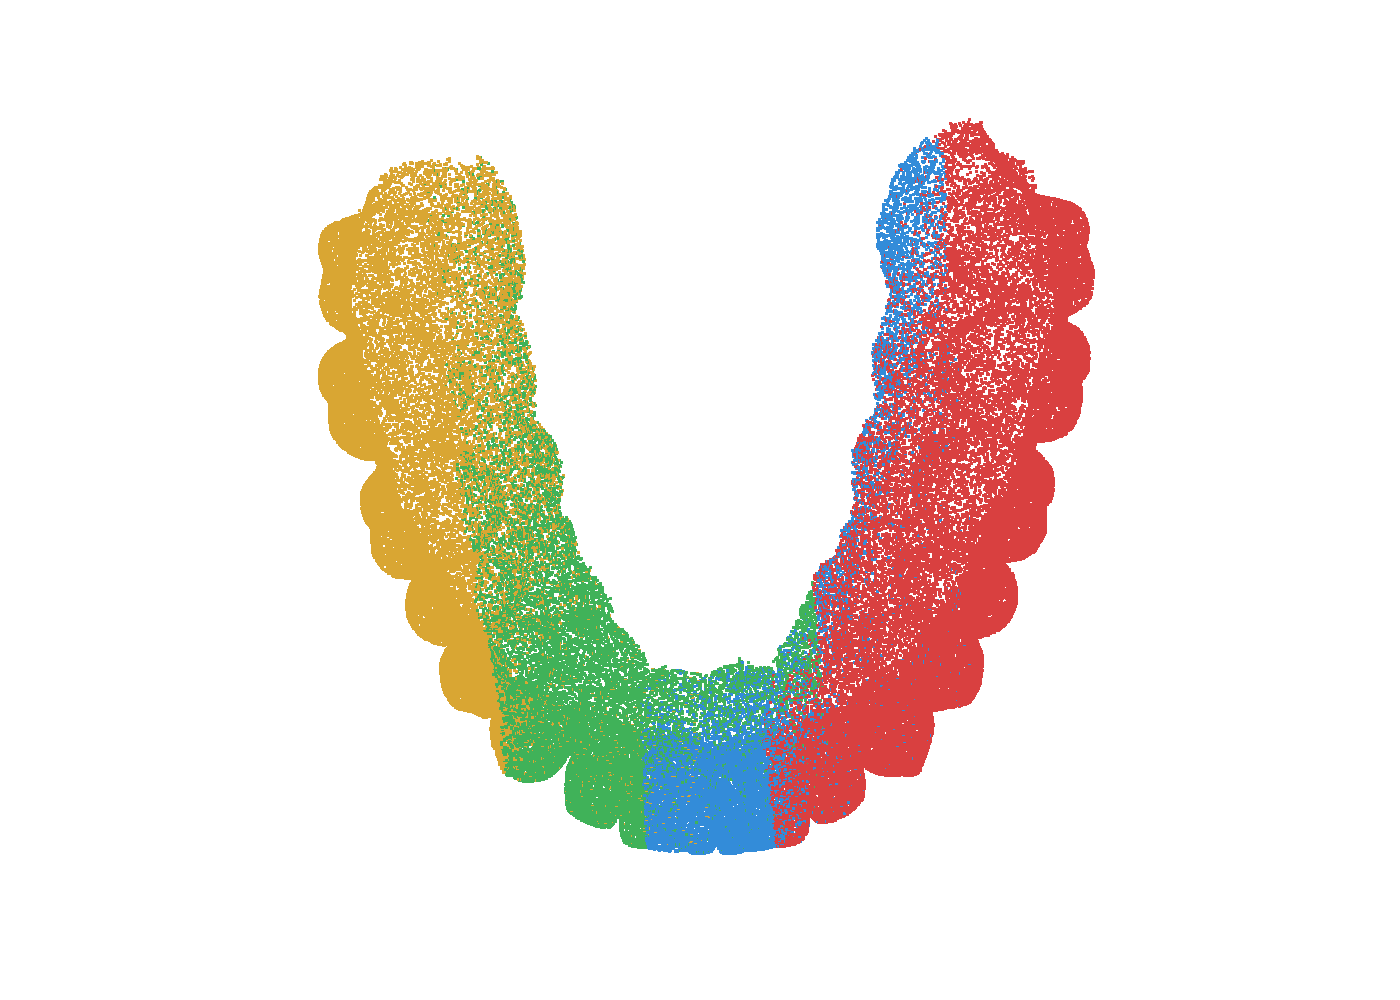
\includegraphics[width=\linewidth]{assets/marvin/upper_registered.png}
    \caption{Registered fragments.}
\end{subfigure}
\caption{Representative qualitative example from Model~1. The quantitative registration experiments use all five model sets and all ten jaw meshes.}
\label{fig:realistic-representative-registration}
\end{figure*}

\subsubsection{Pairwise Comparison Across 30 Fragment Pairs}

The same five registration algorithms and preprocessing parameters were applied to the adjacent fragment pairs $0\rightarrow1$, $1\rightarrow2$, and $2\rightarrow3$ for every jaw. This yields 30 geometrically distinct zero-noise pairwise cases. Success requires translation error $\leq1$ model unit and rotation error $\leq1^\circ$.

\begin{table*}[!t]
\centering
\footnotesize
\setlength{\tabcolsep}{4pt}
\begin{tabular}{lrrrrrr}
\toprule
\textbf{Method} & \textbf{Success} & \textbf{Mean $e_t$} & \textbf{Median $e_t$} & \textbf{Mean $e_R$ [$^\circ$]} & \textbf{Median $e_R$ [$^\circ$]} & \textbf{Runtime [s]} \\
\midrule
Point-to-Point ICP & 50.0\% & 2.395165 & 0.226672 & 8.768677 & 0.899657 & 0.283623 \\
Point-to-Plane ICP & 80.0\% & 1.842892 & 0.013040 & 6.905271 & 0.070498 & 0.131327 \\
Generalized ICP & 73.3\% & 1.632389 & 0.001382 & 8.141821 & 0.008669 & 0.141021 \\
FPFH + FGR + ICP & 73.3\% & 3.977360 & 0.001573 & 10.316597 & 0.010267 & 0.891728 \\
\textbf{FPFH + RANSAC + ICP} & \textbf{100.0\%} & \textbf{0.001921} & \textbf{0.001509} & \textbf{0.009483} & \textbf{0.009741} & 0.681506 \\
\bottomrule
\end{tabular}
\caption{Pairwise registration summary across 30 adjacent fragment pairs from ten jaw meshes. Large mean-to-median gaps for several competing methods are caused by catastrophic registration failures.}
\label{tab:realistic-pairwise-summary}
\end{table*}

\begin{figure*}[!t]
\centering
\begin{subfigure}[t]{0.48\textwidth}
    \centering
    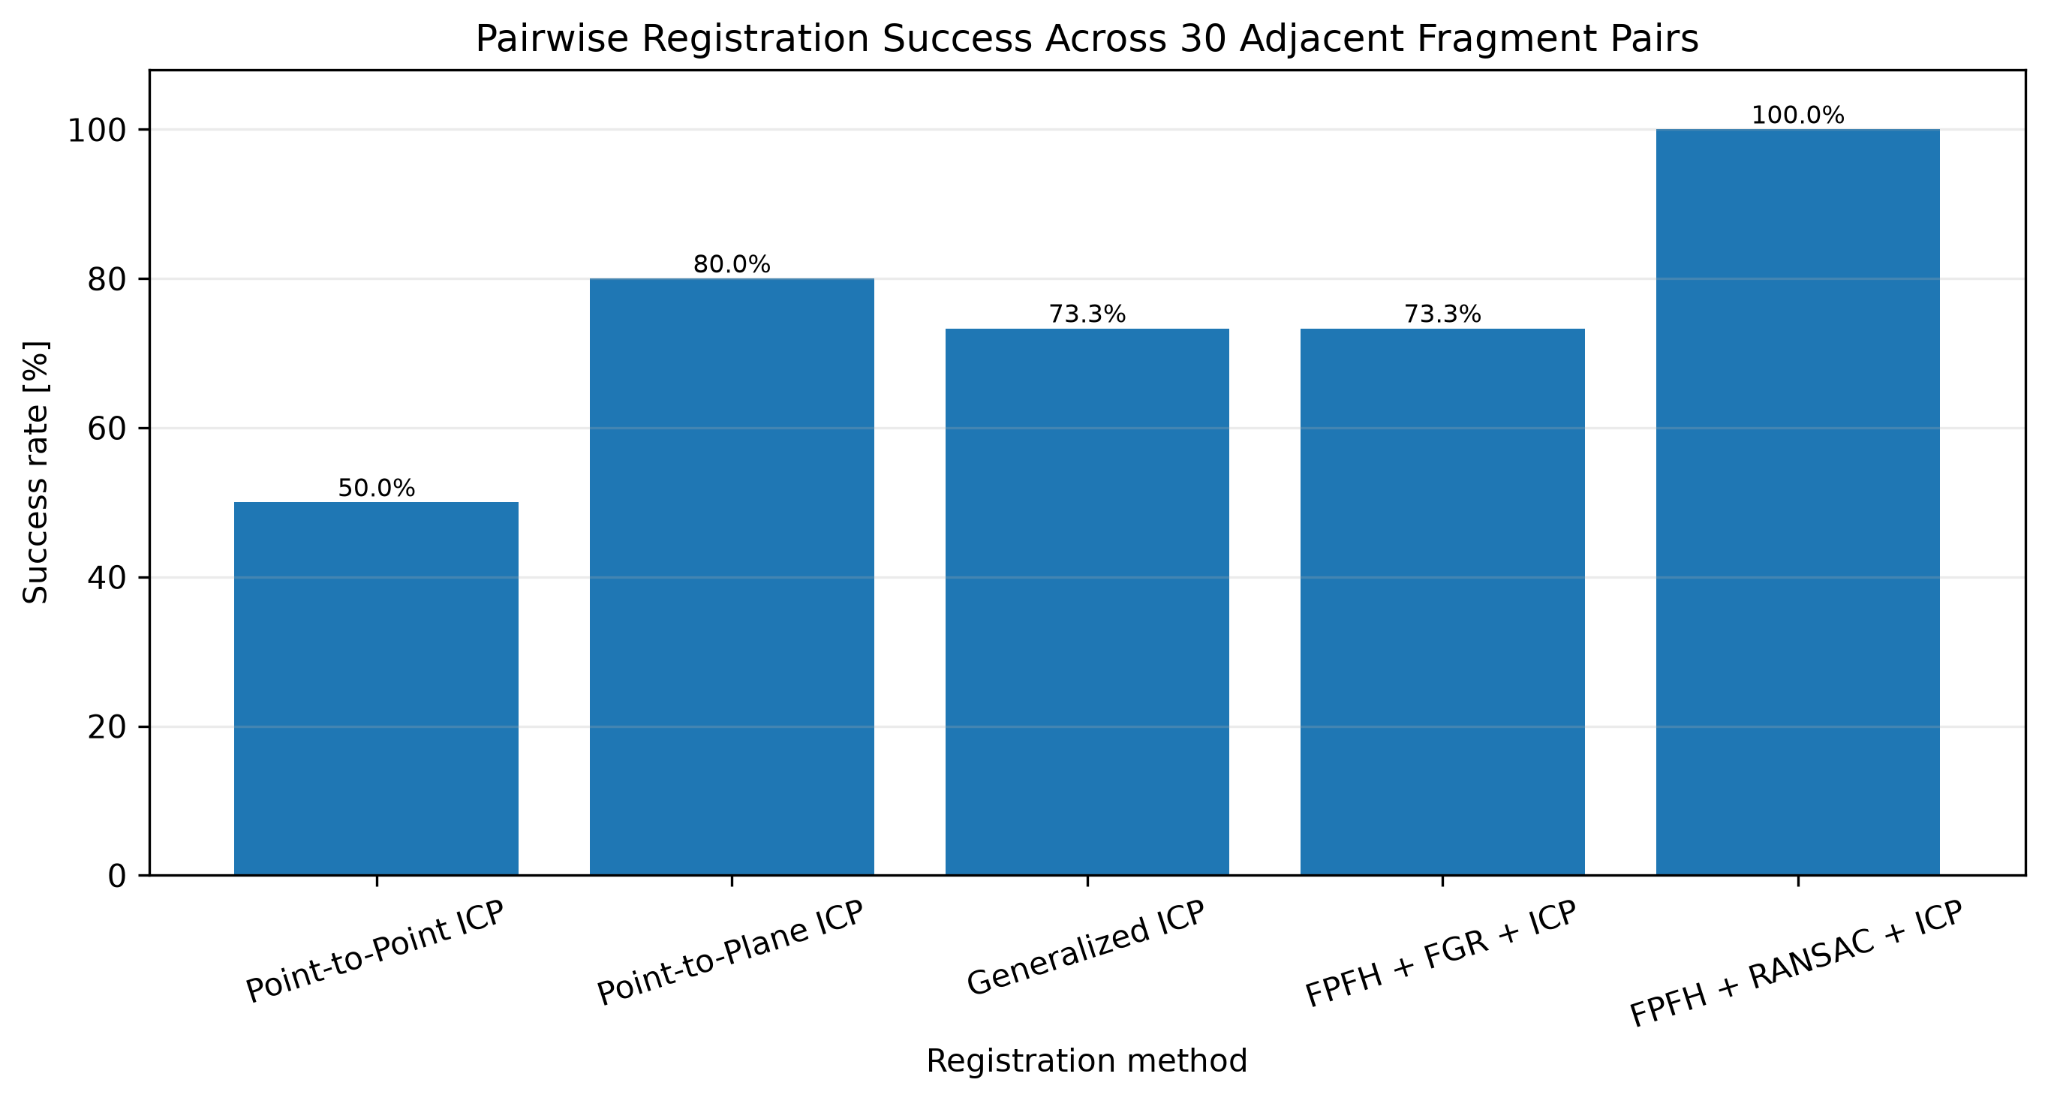
\includegraphics[width=\linewidth]{assets/marvin/model_suite/model_suite_pairwise_success_rate.png}
    \caption{Overall success across 30 cases.}
\end{subfigure}\hfill
\begin{subfigure}[t]{0.48\textwidth}
    \centering
    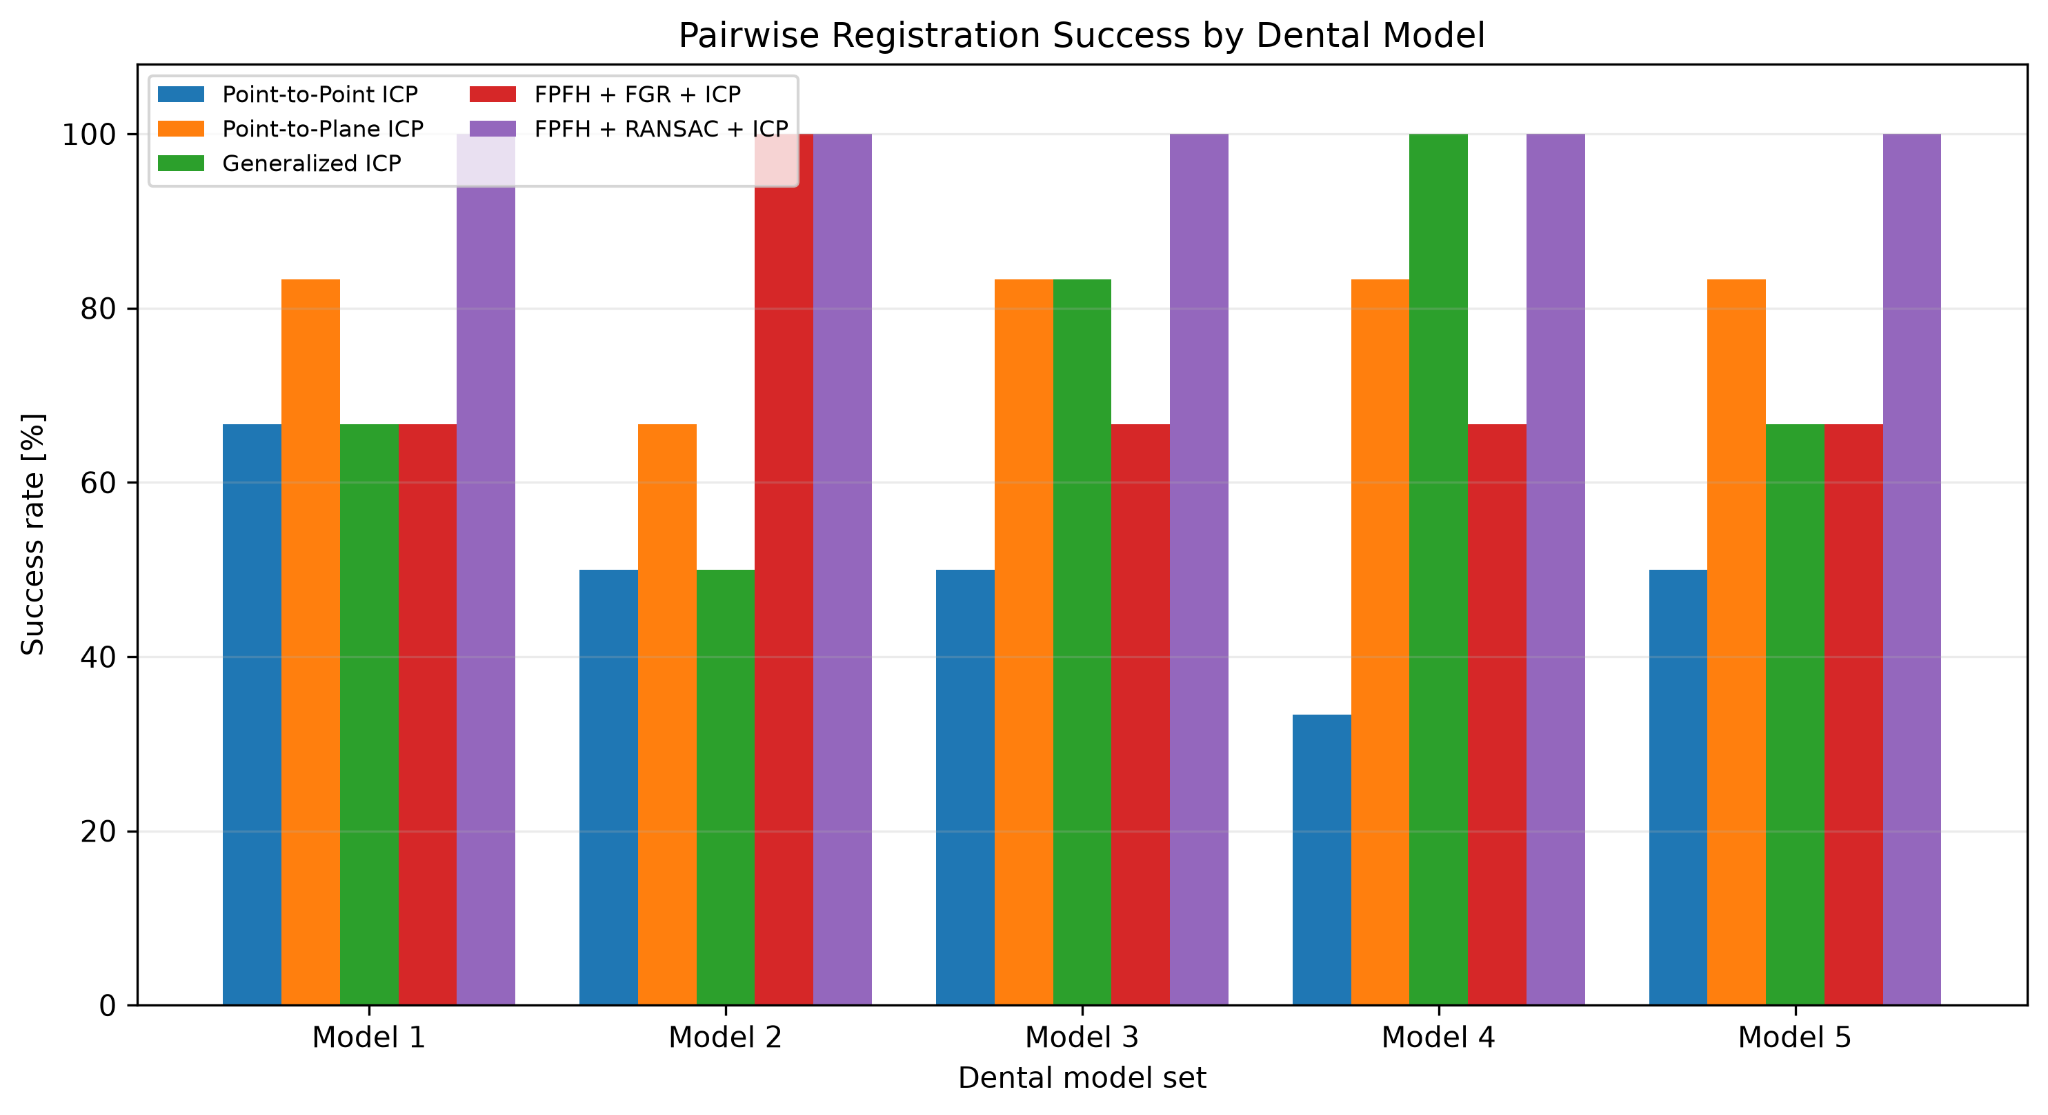
\includegraphics[width=\linewidth]{assets/marvin/model_suite/model_suite_pairwise_success_by_model.png}
    \caption{Success separated by model set.}
\end{subfigure}
\caption{Five-model zero-noise pairwise validation. RANSAC + ICP achieved 30/30 successful registrations and 100\% success in every individual model set.}
\label{fig:model-suite-pairwise}
\end{figure*}

The five-model experiment makes the distinction between precision and robustness particularly clear. FGR + ICP and GICP have very small median errors when they converge correctly, yet their much larger mean errors reveal severe outliers. RANSAC + ICP combines similarly low successful-case error with no failures in the 30 evaluated adjacent-fragment cases. The 100\% observed rate corresponds to 30/30 cases and is reported as a benchmark result rather than as evidence of universal reliability.


\begin{figure}[!t]
    \centering
    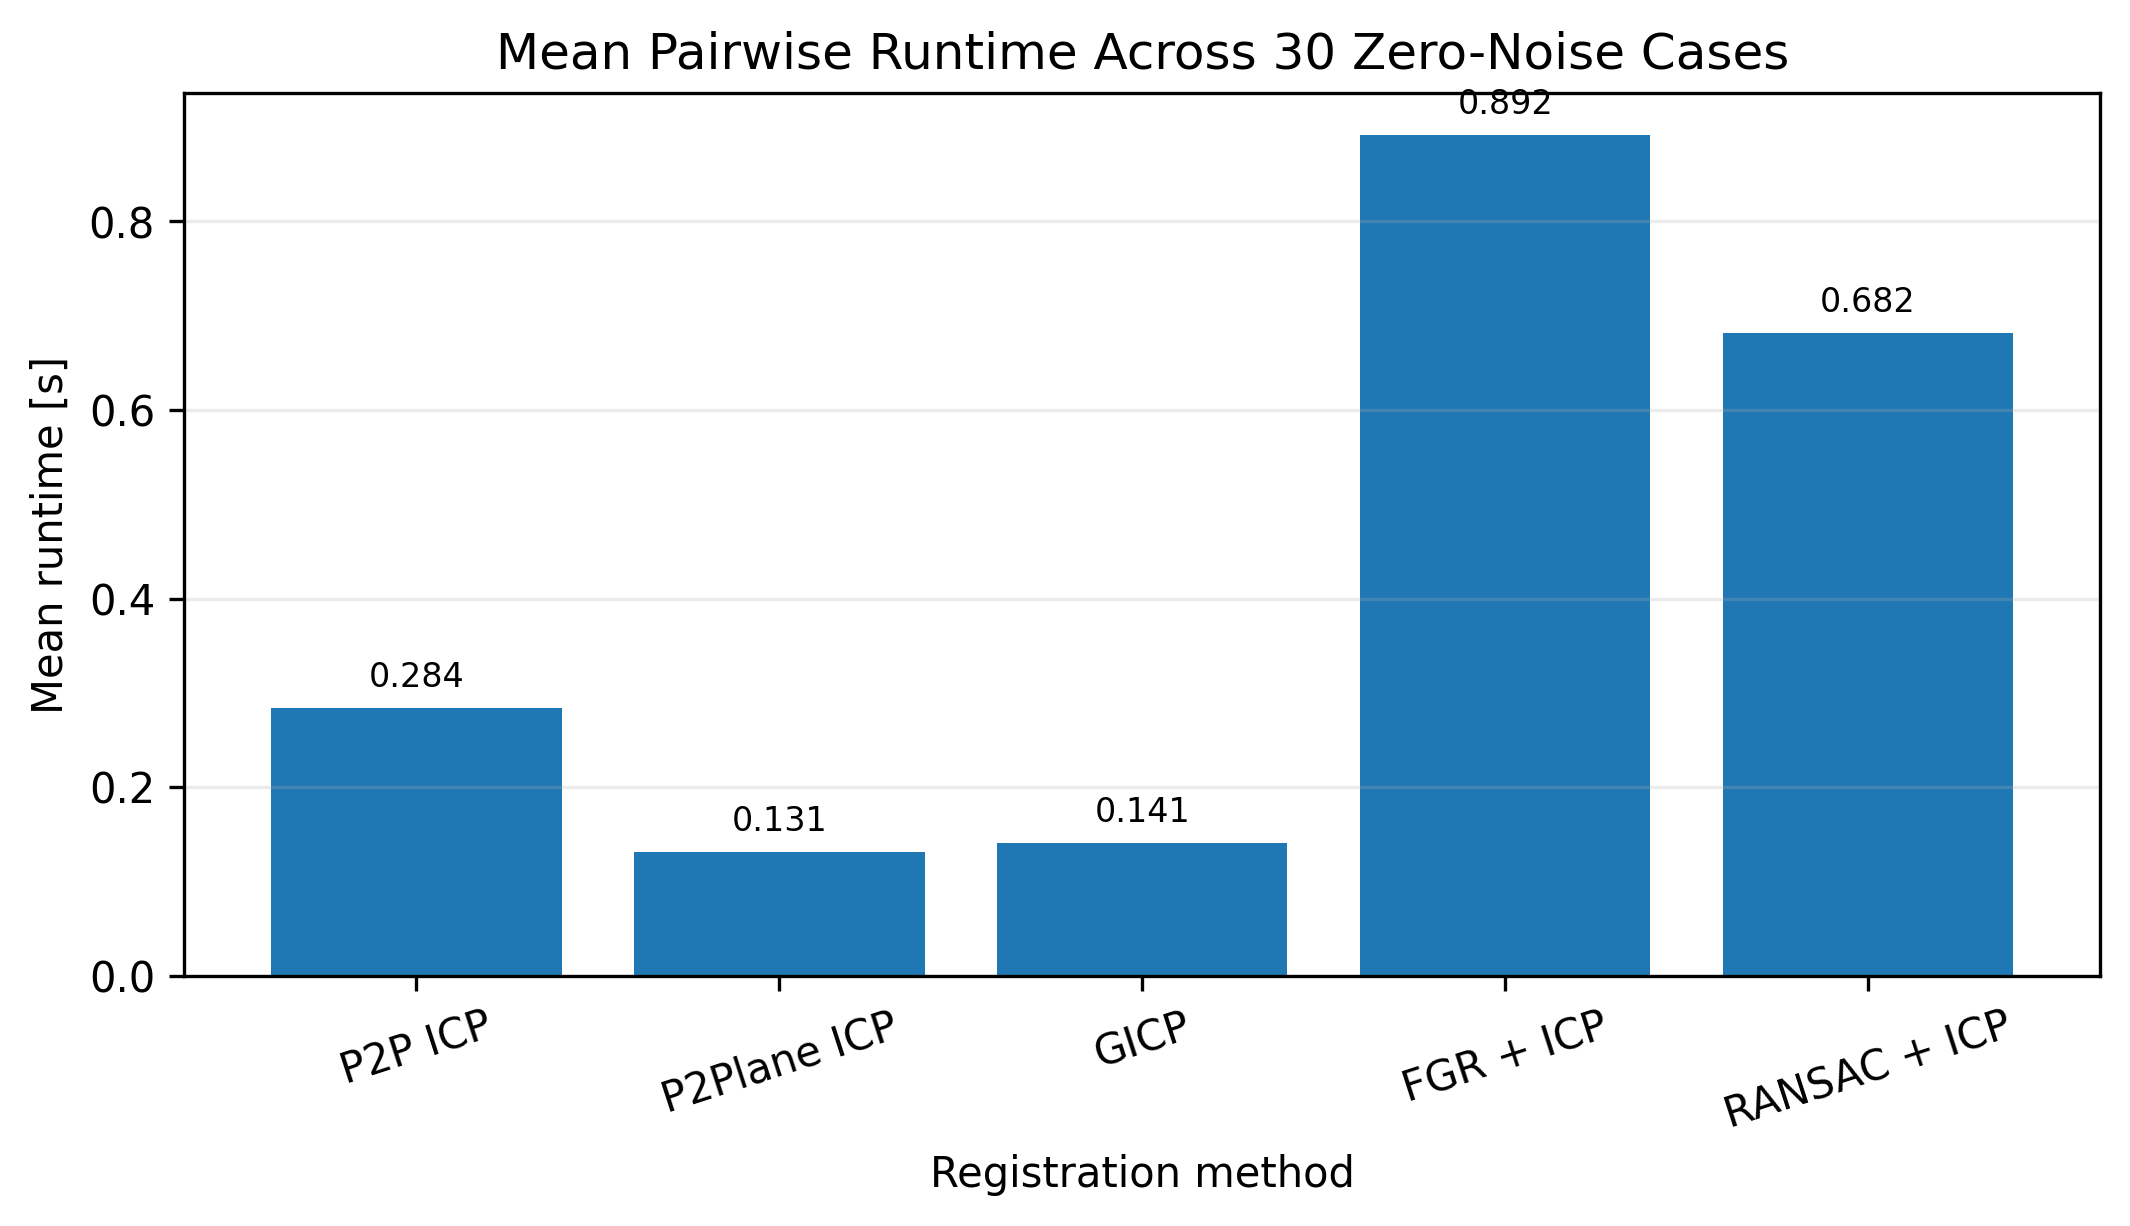
\includegraphics[width=\columnwidth]{assets/marvin/model_suite/model_suite_pairwise_runtime.png}
    \caption{Mean runtime per zero-noise adjacent-pair registration across the 30 realistic cases. The selected RANSAC pipeline is slower than the local ICP variants but remains below FGR in this benchmark while providing substantially higher robustness.}
    \label{fig:model-suite-runtime}
\end{figure}

Runtime therefore represents a real but acceptable trade-off rather than a hidden cost. Point-to-Plane ICP and GICP are fastest at approximately 0.13--0.14~s per evaluated pair, whereas RANSAC + ICP requires about 0.68~s and FGR + ICP about 0.89~s on the benchmark system. The selected RANSAC pipeline is roughly five times slower than the fastest local methods, but those local methods fail on 20--27\% of the zero-noise cases. Since a failed global alignment propagates directly into the subsequent multiway reconstruction, robustness was prioritized over sub-second differences in pairwise runtime.

\subsubsection{Noise Robustness Across Five Models}

Additive isotropic Gaussian positional noise was applied with standard deviations $0$, $0.01$, $0.025$, $0.05$, $0.10$, and $0.20$. At $\sigma=0$, each of the 30 distinct pairwise cases was evaluated once. At every nonzero level, three independent noise realizations were generated for each case, yielding 90 trials per algorithm and noise level. Within a given realization, all algorithms receive exactly the same noisy point clouds.

\begin{figure*}[!t]
    \centering
    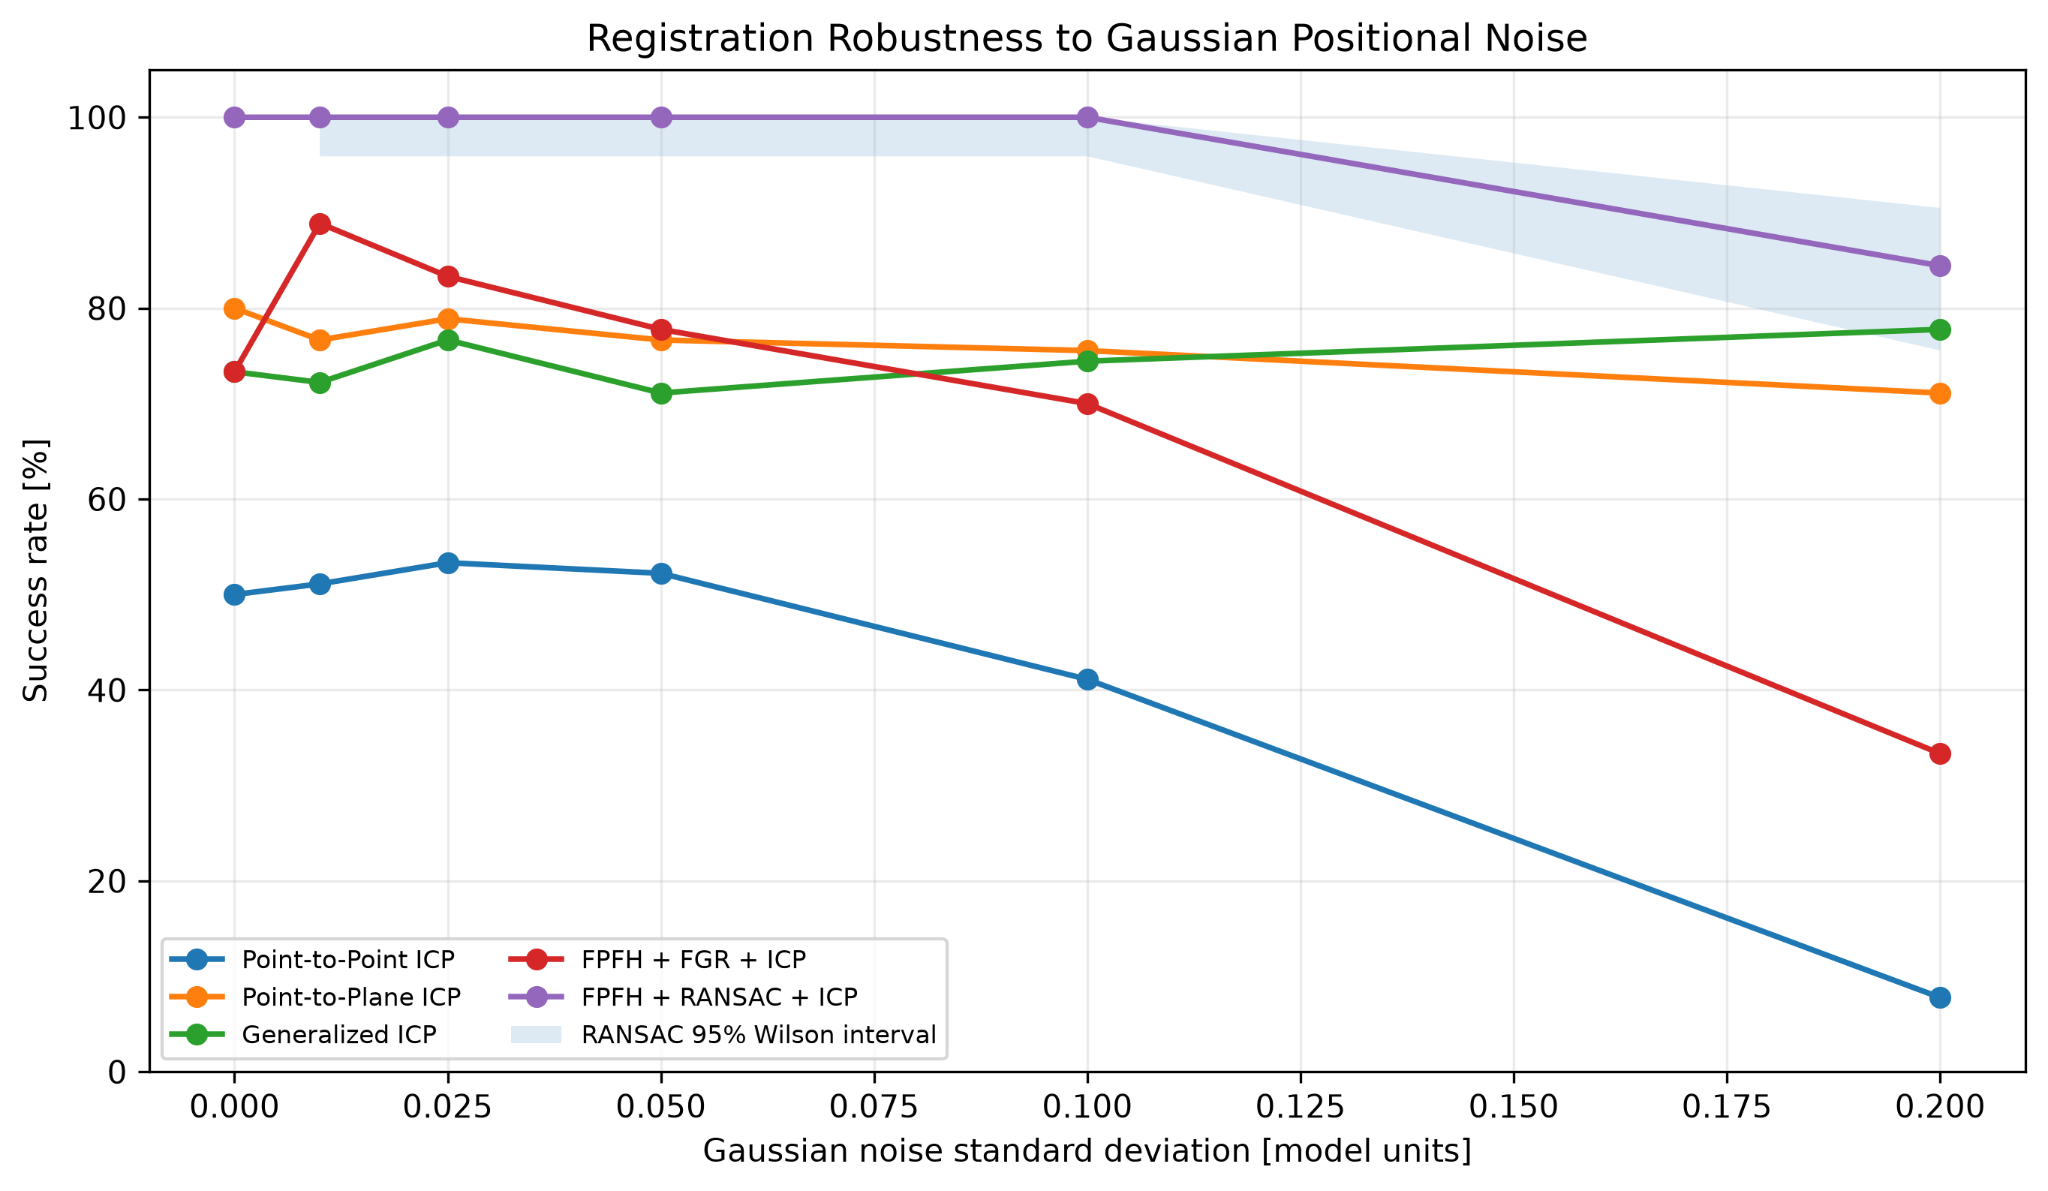
\includegraphics[width=0.82\textwidth]{assets/marvin/model_suite/model_suite_noise_success_rate.png}
    \caption{Success rate under additive Gaussian positional noise across five dental model sets. The shaded band shows the 95\% Wilson interval for RANSAC + ICP at nonzero noise levels. Because repeated noise realizations share the same 30 underlying fragment pairs, the intervals are used as descriptive finite-sample uncertainty indicators rather than formal population-level confidence statements.}
    \label{fig:model-suite-noise}
\end{figure*}

\begin{table}[H]
\centering
\footnotesize
\setlength{\tabcolsep}{3pt}
\begin{tabular}{rrrrrr}
\toprule
$\sigma$ & \textbf{P2P} & \textbf{P2Plane} & \textbf{GICP} & \textbf{FGR} & \textbf{RANSAC} \\
\midrule
0.000 & 50.0 & 80.0 & 73.3 & 73.3 & \textbf{100.0} \\
0.010 & 51.1 & 76.7 & 72.2 & 88.9 & \textbf{100.0} \\
0.025 & 53.3 & 78.9 & 76.7 & 83.3 & \textbf{100.0} \\
0.050 & 52.2 & 76.7 & 71.1 & 77.8 & \textbf{100.0} \\
0.100 & 41.1 & 75.6 & 74.4 & 70.0 & \textbf{100.0} \\
0.200 & 7.8 & 71.1 & 77.8 & 33.3 & \textbf{84.4} \\
\bottomrule
\end{tabular}
\caption{Success rate [\%] in the five-model noise study. The zero-noise row contains 30 unique cases; every nonzero row contains 90 noisy trials per algorithm.}
\label{tab:model-suite-noise}
\end{table}

RANSAC + ICP remained at 100\% observed success through $\sigma=0.10$. At $\sigma=0.20$, 76 of 90 trials succeeded, corresponding to 84.44\% and a Wilson interval of approximately 75.57--90.50\%. At the same level FGR dropped to 33.3\%, while GICP and Point-to-Plane ICP reached 77.8\% and 71.1\%, respectively. The RANSAC mean translation and rotation errors at $\sigma=0.10$ were only 0.02285 model units and $0.0898^\circ$. At $\sigma=0.20$, the mean errors rose to 0.4002 model units and $2.749^\circ$, whereas the corresponding medians remained much smaller at 0.1634 and $0.522^\circ$. This mean-to-median separation indicates that the strongest-noise condition is dominated by a subset of catastrophic failures rather than by a uniform loss of precision.


A second non-monotonic effect appears for FGR at very low noise: its observed success rate rises from 73.3\% at $\sigma=0$ to 88.9\% at $\sigma=0.01$ before decreasing again as the perturbation grows. This should not be interpreted as evidence that additive noise generally improves FGR. A plausible dataset-specific explanation is that small perturbations slightly change local neighborhoods and therefore FPFH descriptors, which can disrupt ambiguous feature correspondences produced by repetitive dental geometry and occasionally move the global optimization toward a more favorable hypothesis. At larger noise levels, descriptor degradation dominates and performance declines. Because the 90 nonzero-noise trials are repeated perturbations of the same 30 base pairs, this pattern is treated as a descriptive observation rather than as a statistically independent demonstration of a beneficial-noise effect.

\begin{samepage}
The expanded realistic validation therefore confirms the final pairwise choice:
\begin{center}
\textbf{FPFH $\rightarrow$ RANSAC $\rightarrow$ Point-to-Plane ICP.}
\end{center}
\end{samepage}

\subsection{Multiway Registration}
\label{sec:marvin-multiway}

The selected RANSAC + ICP pipeline was applied sequentially to the four fragments of every jaw. Pairwise transformations were chained into the reference coordinate system of fragment 0 without loop-closure correction, so the experiment directly measures accumulated odometry error. For pairwise transformation $T_{i\rightarrow i+1}$ and global pose $P_i$,
\begin{equation}
    P_{i+1} = P_i T_{i\rightarrow i+1}^{-1}.
\end{equation}
Because all acquisition transformations are known, each chained pose can be compared directly with ground truth.

\begin{figure*}[!t]
\centering
\begin{subfigure}[t]{0.48\textwidth}
    \centering
    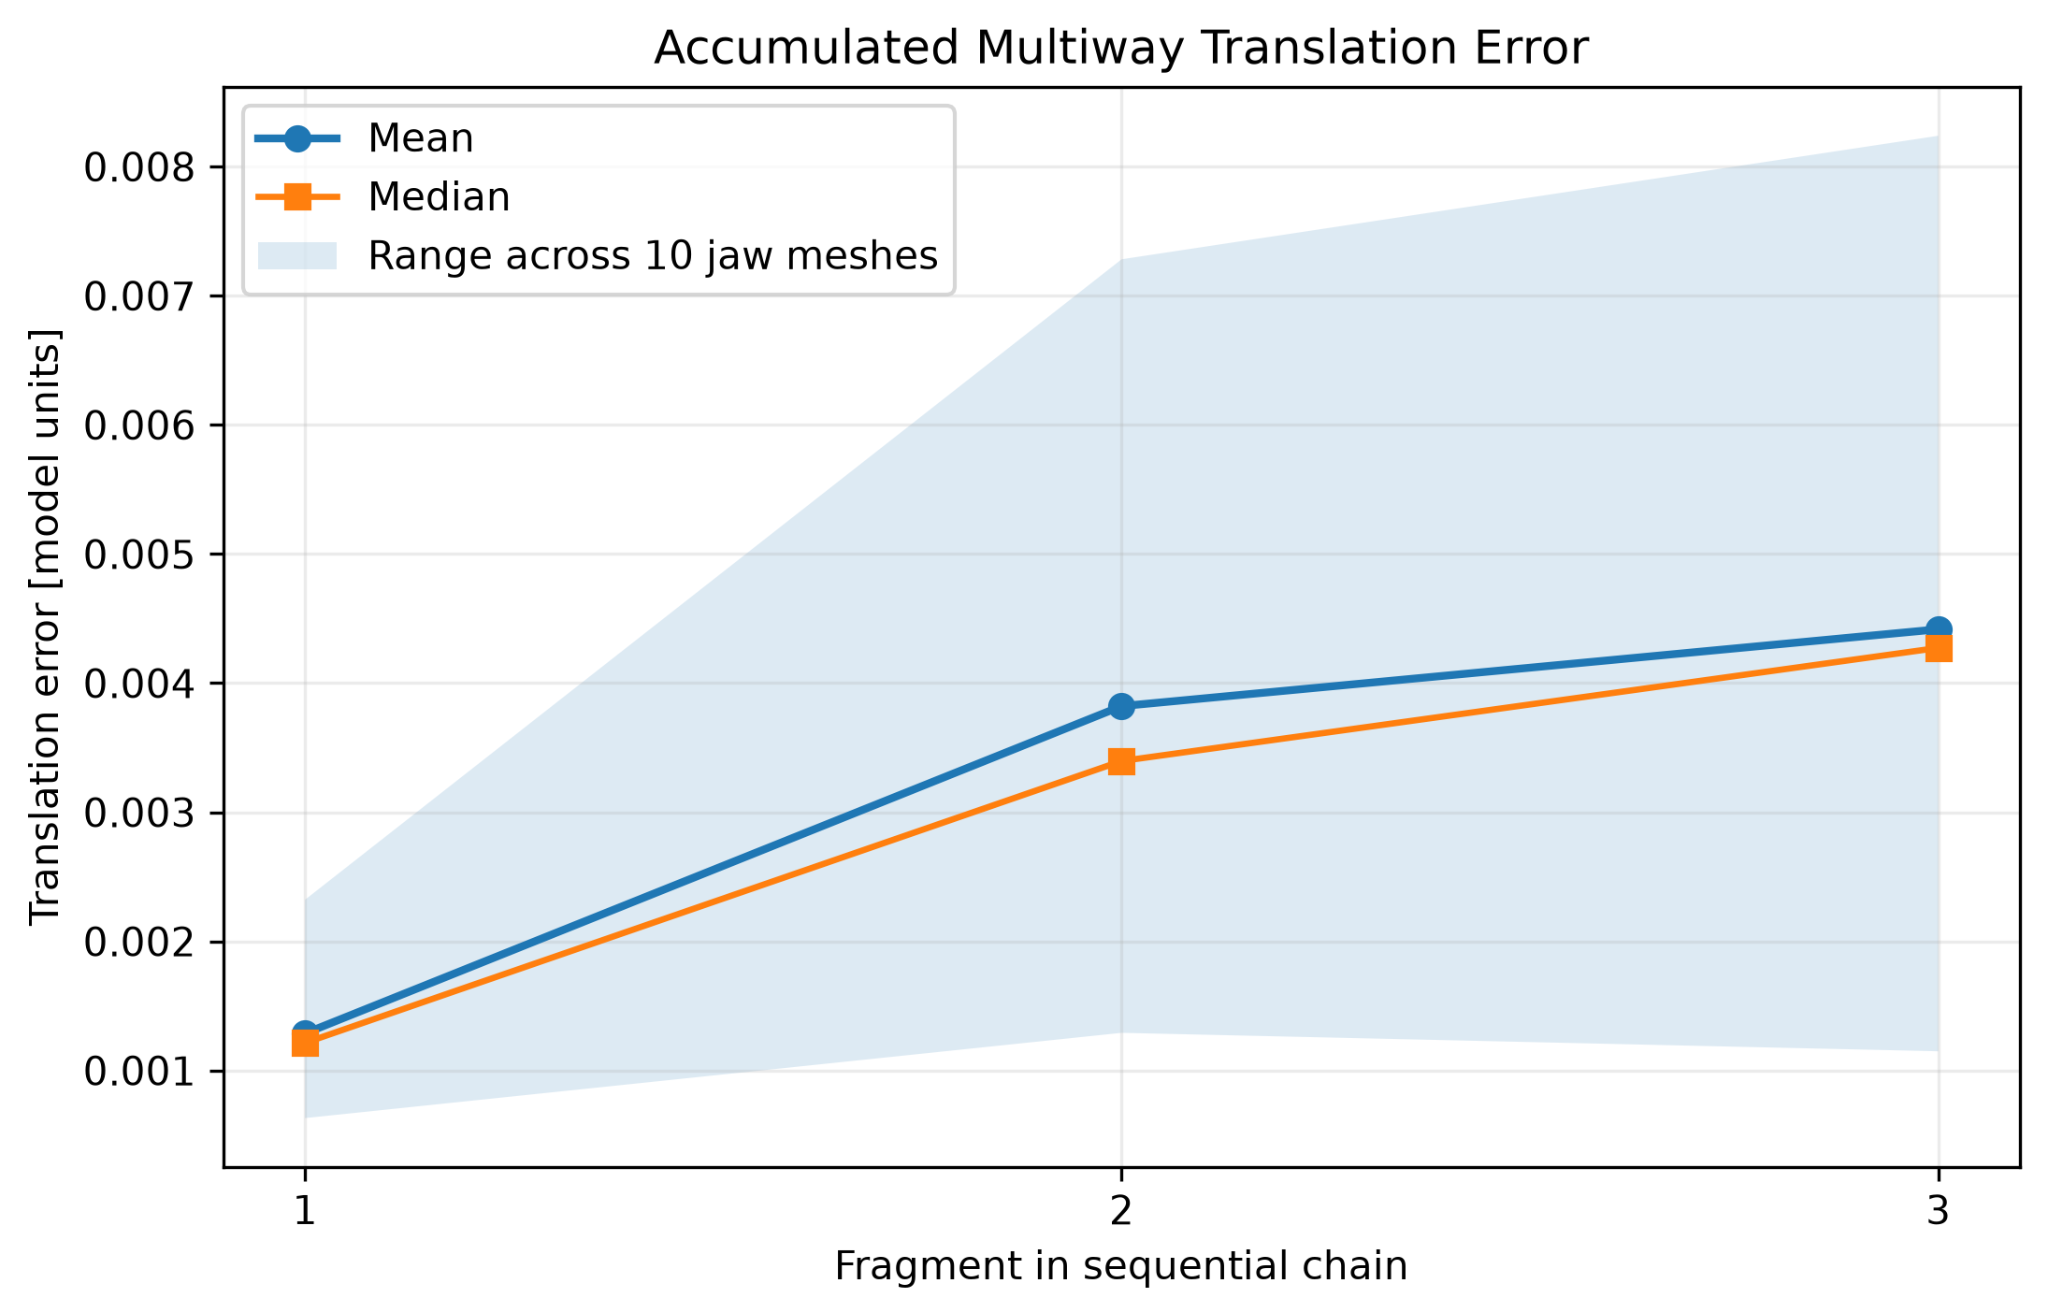
\includegraphics[width=\linewidth]{assets/marvin/model_suite/model_suite_multiway_translation_error.png}
    \caption{Accumulated translation error.}
\end{subfigure}\hfill
\begin{subfigure}[t]{0.48\textwidth}
    \centering
    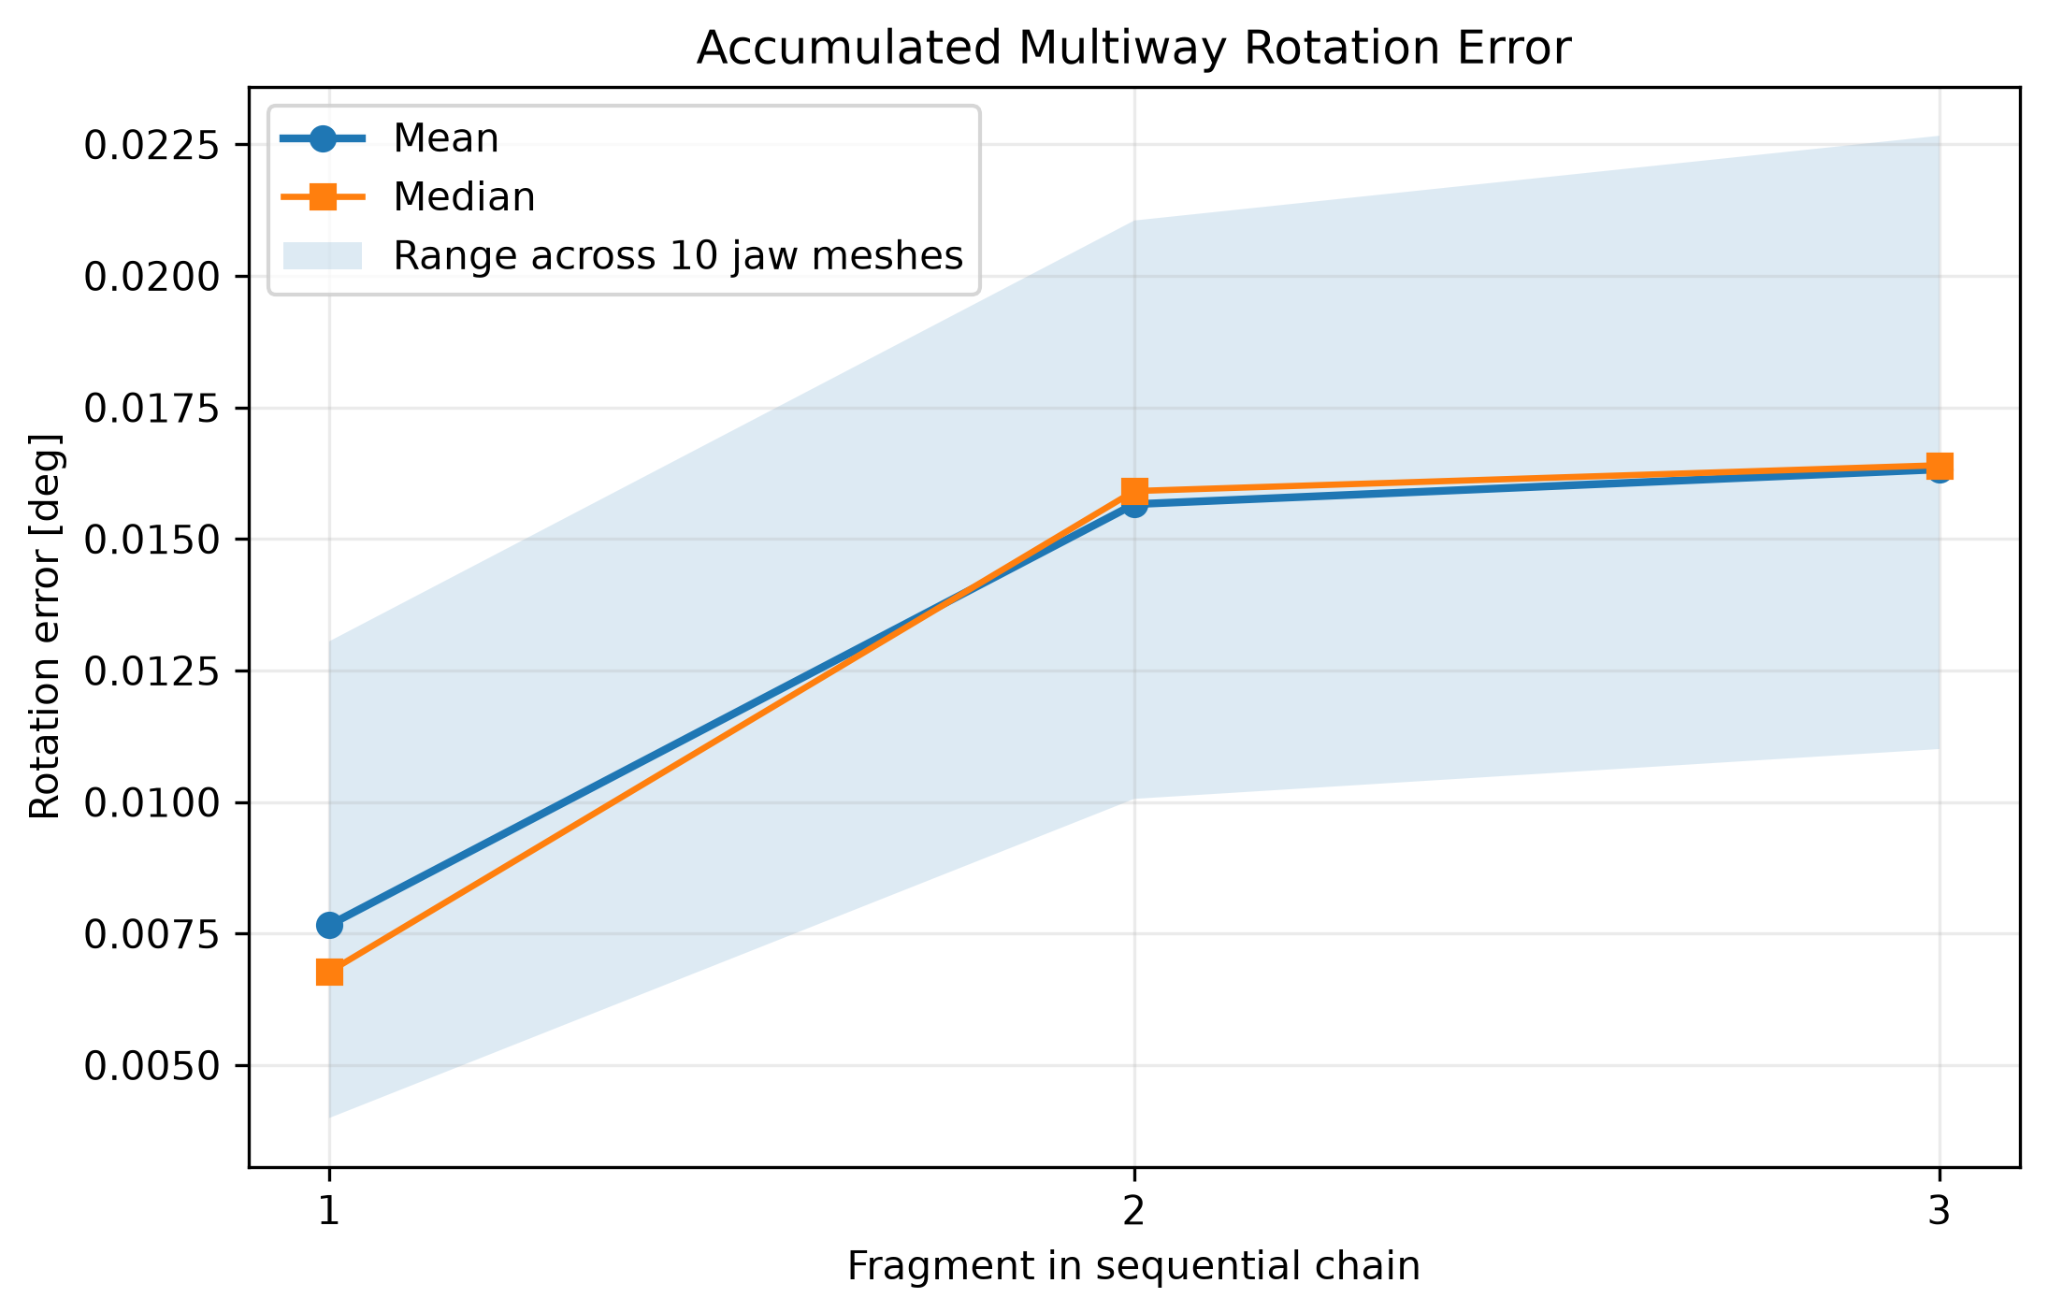
\includegraphics[width=\linewidth]{assets/marvin/model_suite/model_suite_multiway_rotation_error.png}
    \caption{Accumulated rotation error.}
\end{subfigure}
\caption{Sequential multiway error across all ten jaw meshes. Lines show mean and median; shaded regions show the full range across the ten jaws.}
\label{fig:model-suite-multiway-errors}
\end{figure*}

\begin{table}[H]
\centering
\footnotesize
\begin{tabularx}{\columnwidth}{@{}lYYY@{}}
\toprule
\textbf{Metric} & \textbf{Mean} & \textbf{Median} & \textbf{Maximum} \\
\midrule
Translation error [model units] & 0.003175 & 0.003059 & 0.008239 \\
Rotation error [$^\circ$] & 0.013212 & 0.013768 & 0.022660 \\
\bottomrule
\end{tabularx}
\caption{Global pose error over 30 non-reference poses from ten sequential four-fragment registrations.}
\label{tab:model-suite-multiway-overall}
\end{table}

The pairwise middle edge $1\rightarrow2$ remains the most difficult odometry step across the model suite: its mean pairwise rotation error is $0.01310^\circ$, compared with $0.00766^\circ$ for $0\rightarrow1$ and $0.00758^\circ$ for $2\rightarrow3$. Even after sequential accumulation, however, the worst observed global pose error remains only 0.008239 model units in translation and $0.02266^\circ$ in rotation. The ten merged point clouds form the inputs to the surface-reconstruction validation.

\subsection{Surface Reconstruction}
\label{sec:marvin-surface-reconstruction}

A point cloud contains discrete surface samples but no explicit connectivity \cite{kraus_huang2024}. The model-construction stage therefore estimates a triangular surface from the registered points. Two methods were compared: Poisson Surface Reconstruction \cite{kraus_kazhdan2006} and the Ball Pivoting Algorithm \cite{kraus_bernardini1999}.

Poisson reconstruction solves for an implicit surface and tends to produce smooth, globally connected geometry. This is advantageous for completeness, but missing measurements may be bridged by surfaces that are not actually supported by the input points. Ball Pivoting constructs triangles locally by rolling virtual balls with specified radii over the oriented point cloud. It is therefore more conservative but may leave open boundaries when the selected radii are too small.

Normals are estimated using a radius equal to three times the mean nearest-neighbor distance and at most 50 neighbors. Poisson is evaluated at depth 9 with the lowest 2\% density vertices removed. BPA uses multiple radii relative to the mean point spacing.

For mesh evaluation, 100,000 points are sampled uniformly from the reconstructed surface. Distances are measured in both directions: input/reference $\rightarrow$ reconstructed mesh and reconstructed mesh $\rightarrow$ input/reference. The second direction is important because it reveals unsupported surface patches. The symmetric RMSE combines both directions:
\begin{equation}
    \mathrm{RMSE}_{sym} =
    \sqrt{\frac{\mathrm{RMSE}_{A\rightarrow B}^{2}+
    \mathrm{RMSE}_{B\rightarrow A}^{2}}{2}}.
\end{equation}
This is a sampling-based surface approximation rather than an exact point-to-triangle Hausdorff distance.

\begin{figure*}[!t]
\centering
\begin{tikzpicture}[
    node distance=5mm and 7mm,
    box/.style={draw,rounded corners,align=center,minimum width=25mm,minimum height=8mm,font=\footnotesize},
    arr/.style={-{Latex[length=2mm]},thick}
]
\node[box] (cloud) {Registered\\merged cloud};
\node[box, right=of cloud] (norm) {Normal\\estimation};
\node[box, right=of norm] (methods) {Poisson /\\Ball Pivoting};
\node[box, right=of methods] (eval) {Bidirectional\\surface evaluation};
\node[box, below=of methods] (clean) {Cleanup +\\component analysis};
\node[box, left=of clean] (topo) {Topology\\analysis};
\node[box, right=of clean] (simp) {Quadric\\simplification};
\node[box, right=of simp] (export) {PLY / STL\\export};
\draw[arr] (cloud) -- (norm);
\draw[arr] (norm) -- (methods);
\draw[arr] (methods) -- (eval);
\draw[arr] (eval) |- (clean);
\draw[arr] (clean) -- (topo);
\draw[arr] (clean) -- (simp);
\draw[arr] (simp) -- (export);
\end{tikzpicture}
\caption{Surface-reconstruction and model-processing workflow. Algorithm selection is based on geometry and topology rather than visual smoothness alone.}
\label{fig:surface-reconstruction-workflow}
\end{figure*}

\subsection{Synthetic Mesh Evaluation}
\label{sec:marvin-synthetic-mesh}

\subsubsection{Poisson versus Ball Pivoting}

On the synthetic merged cloud containing 22,022 points, Poisson produced a dense surface but also a very large mesh-to-cloud error and self-intersections. The cleaned BPA reconstruction was much closer to the observed geometry.

\begin{table}[!t]
\centering
\footnotesize
\setlength{\tabcolsep}{3pt}
\begin{tabularx}{\columnwidth}{@{}lYY@{}}
\toprule
\textbf{Metric} & \textbf{Poisson} & \textbf{BPA} \\
\midrule
Triangles & 151,430 & 40,020 \\
Connected components & 17 & 1 \\
Self-intersections & Yes & No \\
Cloud $\rightarrow$ mesh RMSE & 0.122208 & 0.076404 \\
Mesh $\rightarrow$ cloud RMSE & 2.741374 & 0.115709 \\
Symmetric RMSE & 1.940369 & 0.098046 \\
\bottomrule
\end{tabularx}
\caption{Synthetic surface-reconstruction comparison after BPA cleanup.}
\label{tab:synthetic-mesh-comparison}
\end{table}

\begin{figure}[!t]
    \centering
    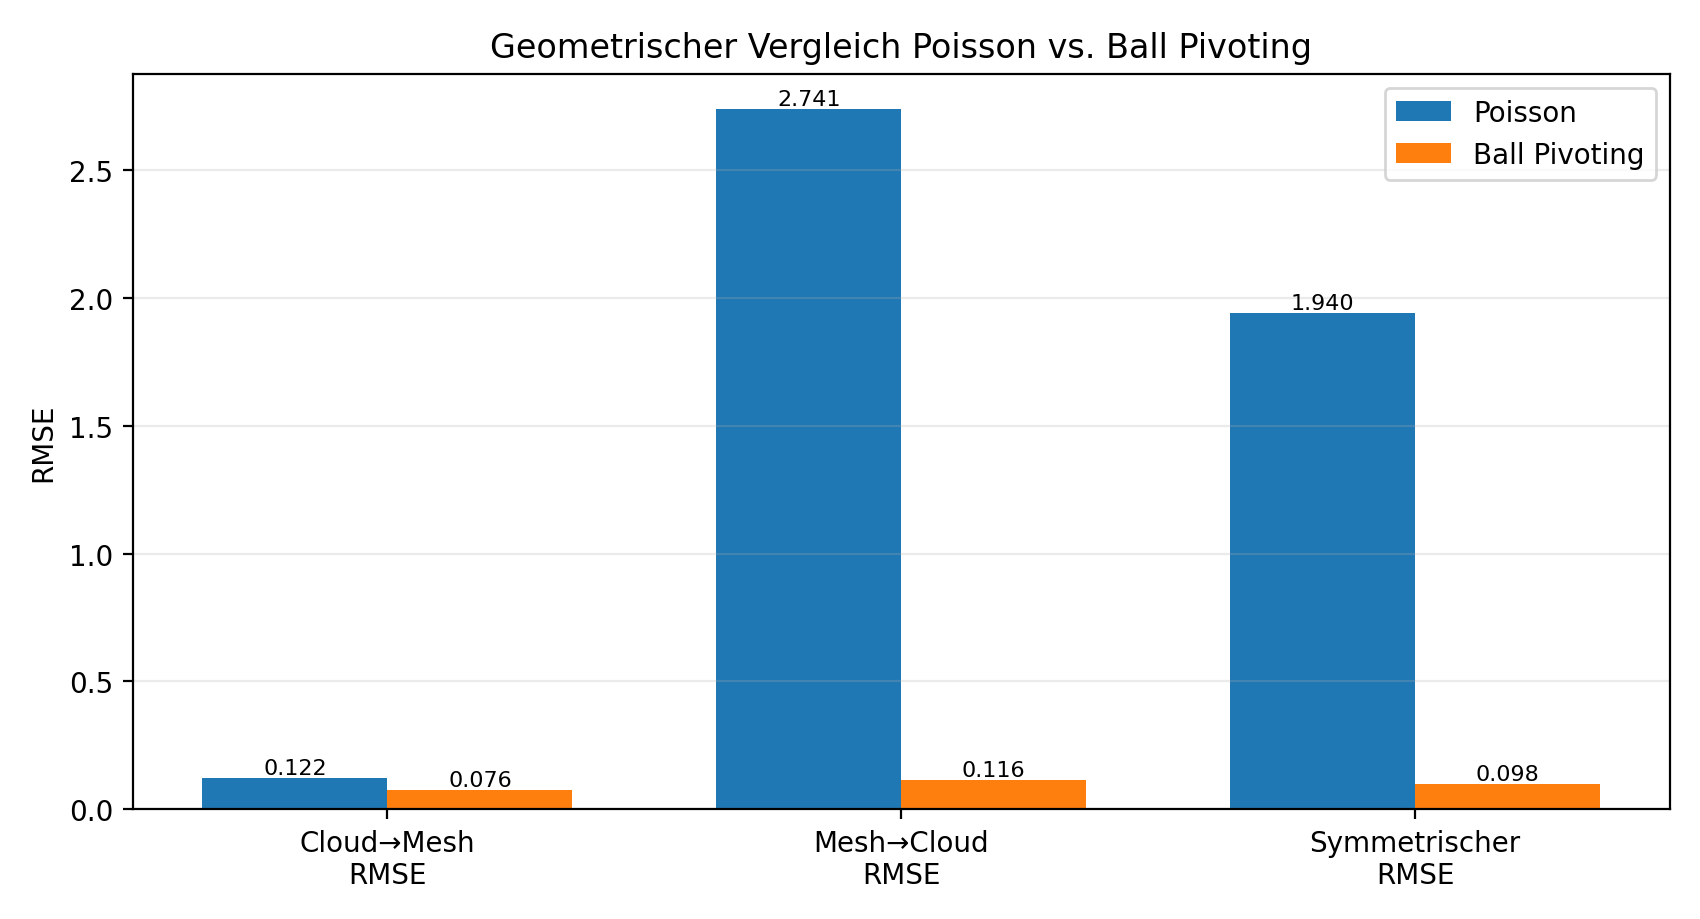
\includegraphics[width=0.92\linewidth]{assets/marvin/poisson_vs_ball_pivoting_rmse.png}
    \caption{Synthetic geometric error comparison between Poisson and Ball Pivoting.}
    \label{fig:synthetic-poisson-bpa}
\end{figure}

\subsubsection{BPA Parameter Study and Cleanup}

Four BPA radius-factor sets were compared. The smallest set $(1.0,1.5,2.0)$ achieved the lowest symmetric RMSE on the synthetic geometry. Although it initially produced 82 connected components, 99.04\% of all triangles belonged to one dominant component; the remaining components were tiny satellites. Removing components below 250 triangles yielded one connected component with 40,020 triangles.

\begin{figure}[!t]
    \centering
    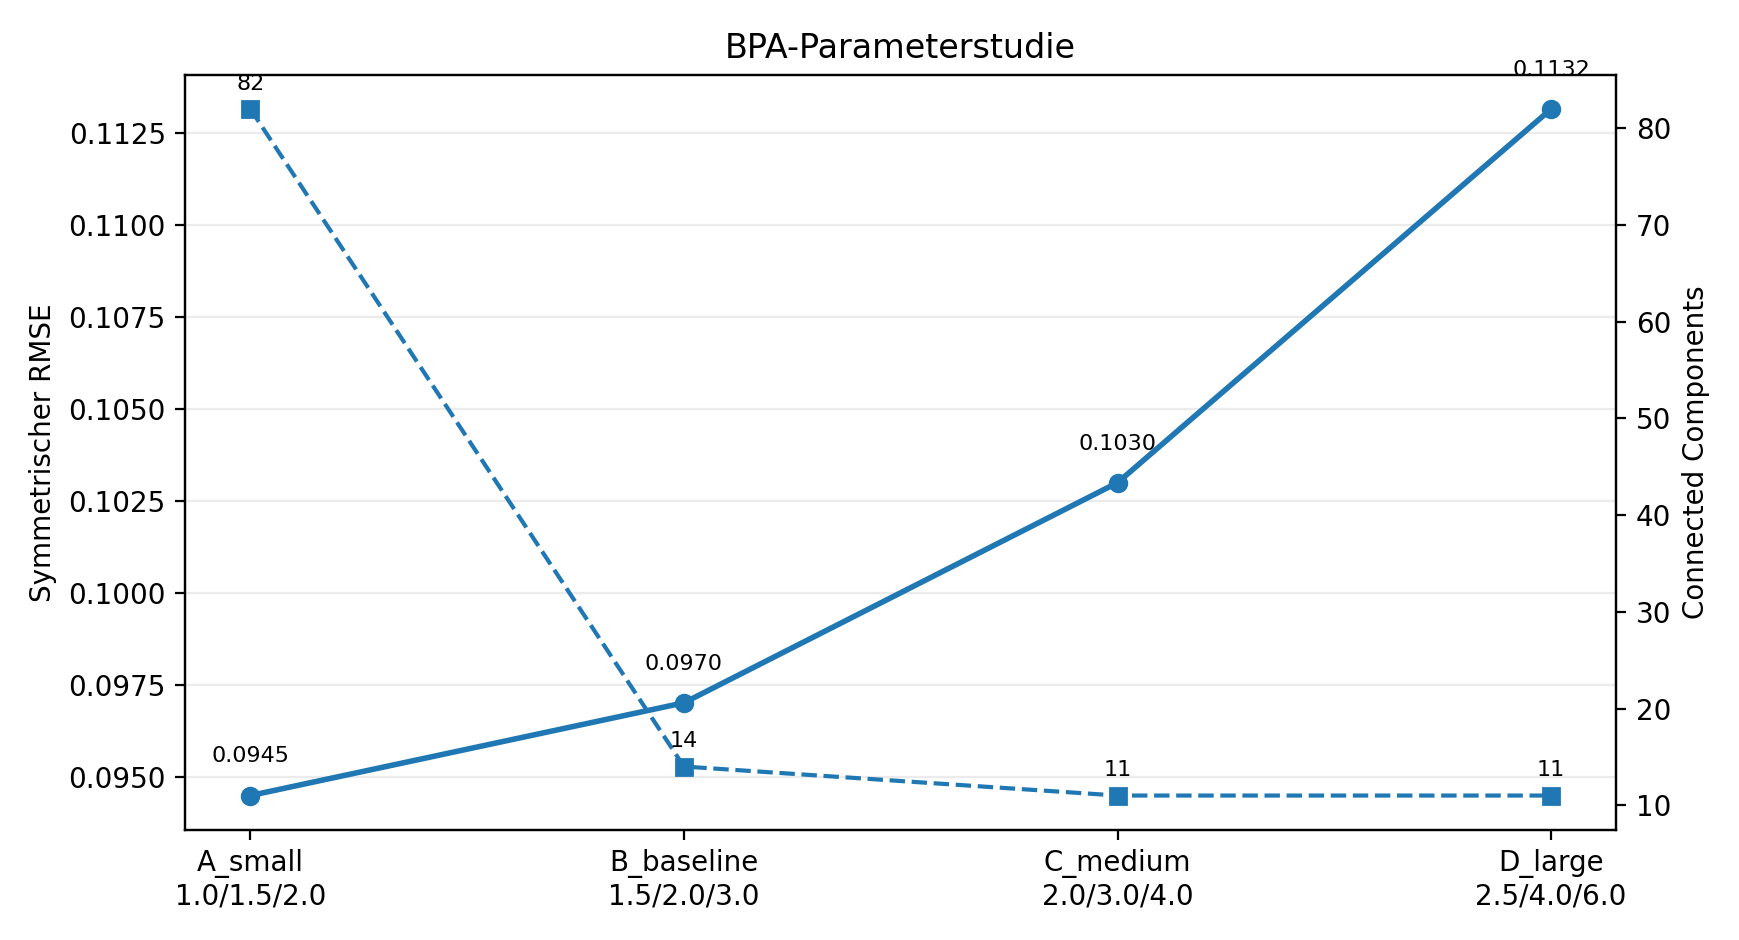
\includegraphics[width=0.92\linewidth]{assets/marvin/bpa_parameter_study.png}
    \caption{Synthetic BPA radius-factor study.}
    \label{fig:synthetic-bpa-study}
\end{figure}

A topology inspection identified no genuine non-manifold edges and no self-intersections, but the surface remained non-watertight, non-vertex-manifold, and globally non-orientable. An attempted vertex-splitting repair removed the non-manifold-vertex condition but introduced self-intersections. The repair was therefore rejected instead of forcing a topologically cleaner but geometrically worse result.

\begin{table}[!t]
\centering
\footnotesize
\begin{tabularx}{\columnwidth}{@{}lY@{}}
\toprule
\textbf{Topology property} & \textbf{Full-resolution BPA candidate} \\
\midrule
Vertices / triangles & 21,689 / 40,020 \\
Boundary edges & 7,982 \\
Non-manifold edges & 0 \\
Non-manifold vertices & 1,204 (5.55\%) \\
Self-intersections & 0 \\
Vertex manifold & No \\
Watertight & No \\
Orientable & No \\
Orientation-conflict edges & 420 \\
Affected triangles & 784 (1.96\%) \\
\bottomrule
\end{tabularx}
\caption{Detailed topology diagnosis of the cleaned synthetic BPA candidate.}
\label{tab:synthetic-topology}
\end{table}

\begin{table}[!t]
\centering
\footnotesize
\begin{tabularx}{\columnwidth}{@{}lYY@{}}
\toprule
\textbf{Property} & \textbf{Original} & \textbf{After vertex splitting} \\
\midrule
Vertices & 21,689 & 22,961 \\
Triangles & 40,020 & 40,020 \\
Non-manifold vertices & 1,204 & 0 \\
Vertex manifold & No & Yes \\
Self-intersections & No & \textbf{Yes} \\
Orientable & No & No \\
Symmetric RMSE & 0.098070 & 0.098070 \\
\bottomrule
\end{tabularx}
\caption{Rejected topology-repair attempt. Removing the non-manifold-vertex condition introduced self-intersections and was therefore not accepted.}
\label{tab:rejected-topology-repair}
\end{table}

\subsubsection{Mesh Simplification}

Quadric decimation \cite{kraus_garland1997} was tested at target sizes of 30,000, 20,000, 10,000, and 5,000 triangles. The 30k variant provided the best compromise: it reduced the triangle count by approximately 25\% while increasing the symmetric RMSE by only 0.171\%.

\begin{figure}[!t]
    \centering
    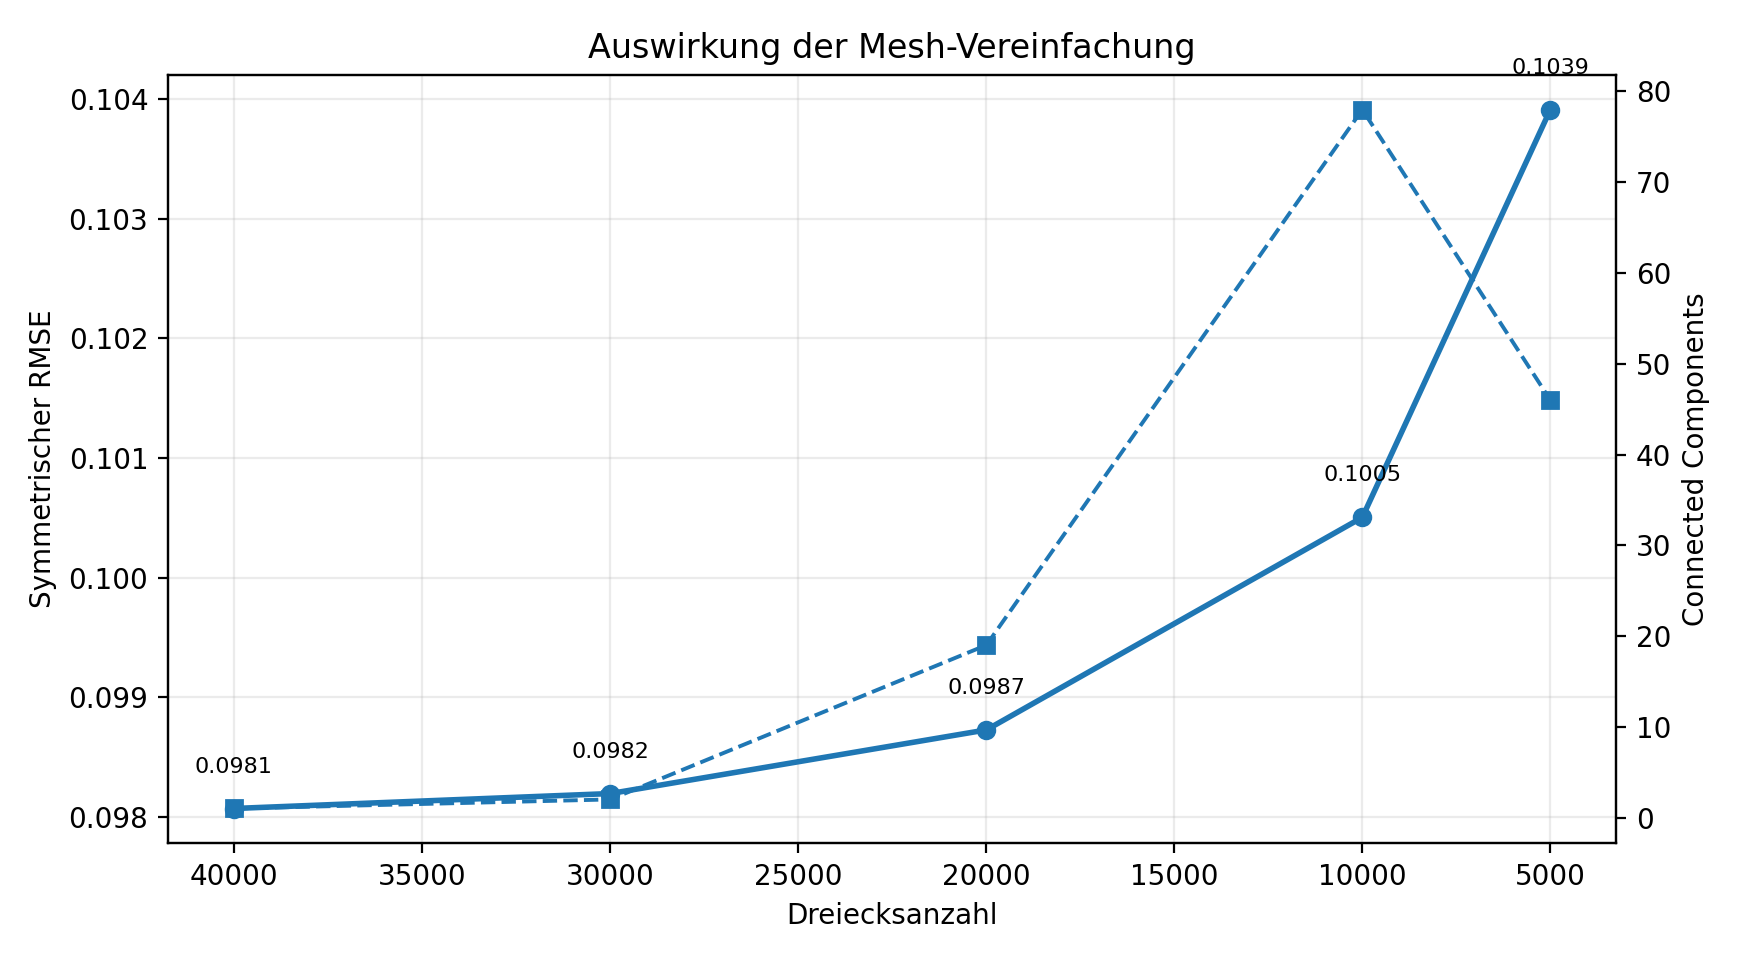
\includegraphics[width=0.92\linewidth]{assets/marvin/mesh_simplification_study.png}
    \caption{Synthetic mesh simplification study.}
    \label{fig:synthetic-simplification}
\end{figure}

\begin{table}[!t]
\centering
\footnotesize
\setlength{\tabcolsep}{3pt}
\begin{tabular}{lrrrr}
\toprule
\textbf{Variant} & \textbf{Triangles} & \textbf{Reduction} & \textbf{Components} & \textbf{Sym. RMSE} \\
\midrule
Original & 40,020 & 0.0\% & 1 & 0.098070 \\
30k & 29,999 & 25.0\% & 2 & 0.098195 \\
20k & 20,000 & 50.0\% & 19 & 0.098727 \\
10k & 10,000 & 75.0\% & 78 & 0.100504 \\
5k & 4,999 & 87.5\% & 46 & 0.103913 \\
\bottomrule
\end{tabular}
\caption{Synthetic simplification study. The 30k variant preserves geometry while stronger simplification rapidly increases fragmentation.}
\label{tab:synthetic-simplification}
\end{table}

After removing one isolated triangle, the final synthetic export contained 16,649 vertices and 29,998 triangles. The symmetric RMSE changed from 0.098070 for the full-resolution cleaned BPA mesh to 0.098237 after simplification and final cleanup, an increase of only 0.171\%. Both PLY and STL exports could be reloaded successfully. PLY reloaded with 16,649 indexed vertices and 29,998 triangles; STL retained the same triangle count but reported more vertices because STL repeats triangle vertices instead of storing the shared indexed connectivity used by PLY. This synthetic export pipeline demonstrates cleanup, simplification, serialization, and integrity checking independently of the later realistic-geometry validation.

\begin{table*}[!t]
\centering
\footnotesize
\begin{tabular}{lrrrrrrr}
\toprule
\textbf{Mesh} & \textbf{Vertices} & \textbf{Triangles} & \textbf{Components} & \textbf{Vertex manifold} & \textbf{Self-int.} & \textbf{Watertight} & \textbf{Sym. RMSE} \\
\midrule
Cleaned full-resolution BPA & 21,689 & 40,020 & 1 & No & No & No & 0.098070 \\
Final 30k export & 16,649 & 29,998 & 1 & No & No & No & 0.098237 \\
\bottomrule
\end{tabular}
\caption{Final synthetic mesh integrity check. Simplification reduces complexity substantially without creating self-intersections or materially changing geometric error.}
\label{tab:final-synthetic-quality}
\end{table*}

The remaining topological limitations are reported rather than hidden by aggressive repair. For visualization and geometric comparison the open BPA surface is acceptable, but applications requiring a closed volume would need a specialized downstream repair stage. This distinction is important for DentaVision: the current contribution targets faithful surface reconstruction, not guaranteed watertight solid modeling.

\subsection{Validation of Surface Reconstruction on Five Dental Models}
\label{sec:marvin-realistic-mesh}

\subsubsection{BPA Radius Re-Optimization Across Ten Jaws}

The realistic BPA parameter study was repeated on all ten registered jaw clouds. Four radius-factor configurations were evaluated against the original STL surfaces using symmetric RMSE, boundary-edge count, component structure, reconstructed-to-reference area ratio, and self-intersections.

\begin{figure*}[!t]
    \centering
    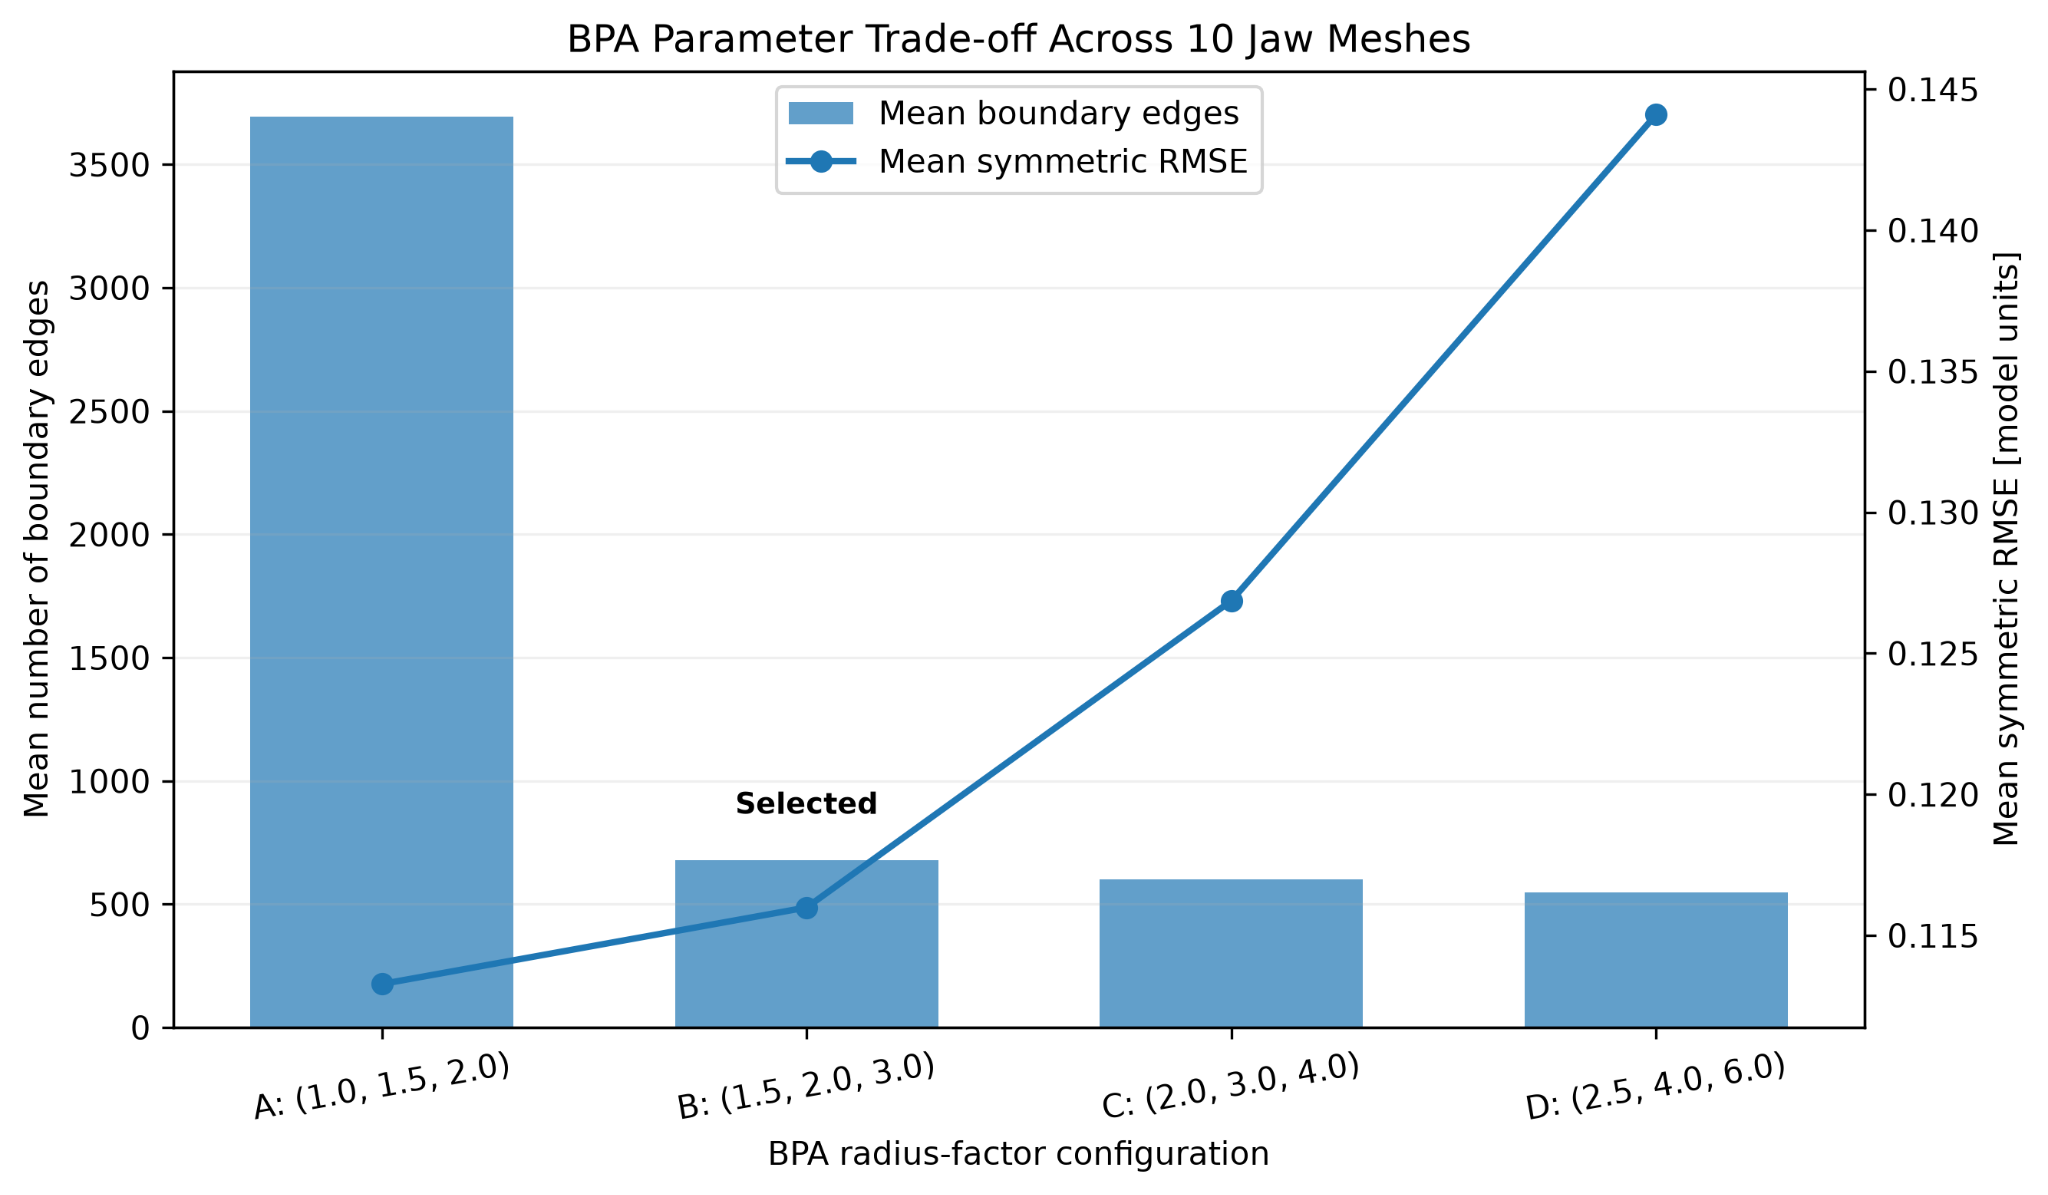
\includegraphics[width=0.84\textwidth]{assets/marvin/model_suite/model_suite_bpa_parameter_tradeoff.png}
    \caption{BPA parameter trade-off across ten jaw meshes. Configuration A minimizes geometric error but leaves many open boundaries. Configuration B is selected as the best compromise between boundary closure and fidelity.}
    \label{fig:model-suite-bpa-tradeoff}
\end{figure*}

\begin{table*}[!t]
\centering
\footnotesize
\setlength{\tabcolsep}{4pt}
\begin{tabular}{lrrrrrr}
\toprule
\textbf{Configuration} & \textbf{Mean sym. RMSE} & \textbf{Mean boundary edges} & \textbf{Mean components} & \textbf{Largest comp. frac.} & \textbf{Mean area ratio} & \textbf{Self-int.} \\
\midrule
A $(1.0,1.5,2.0)$ & \textbf{0.113276} & 3694.1 & 6.0 & 0.998650 & 0.939826 & 0/10 \\
\textbf{B $(1.5,2.0,3.0)$} & 0.115989 & \textbf{678.4} & 3.7 & 0.998970 & \textbf{0.972137} & 0/10 \\
C $(2.0,3.0,4.0)$ & 0.126863 & 600.3 & \textbf{3.2} & \textbf{0.999159} & 0.971531 & 0/10 \\
D $(2.5,4.0,6.0)$ & 0.144096 & 548.1 & 4.3 & 0.998966 & 0.971059 & 0/10 \\
\bottomrule
\end{tabular}
\caption{Aggregate realistic BPA parameter study. Configuration B increases mean symmetric RMSE by only about 2.4\% relative to A while reducing mean boundary edges by about 81.6\%.}
\label{tab:model-suite-bpa-study}
\end{table*}

The same trade-off appears in every model set. Moving from A to B reduces the mean boundary-edge count from 3694.1 to 678.4, while mean symmetric RMSE increases only from 0.113276 to 0.115989. Configurations C and D close only modestly more boundaries than B but increase geometric error by approximately 9.4\% and 24.2\% relative to B. Configuration B is therefore retained as the final realistic BPA setting.

\subsubsection{Poisson versus Final BPA Across Ten Jaws}

Poisson reconstruction and the selected BPA configuration B were then evaluated against all ten original STL surfaces. BPA was more accurate on every model set and produced no self-intersections. Poisson generated fewer open boundaries, but this apparent completeness was achieved by adding large unsupported surface regions.

\begin{table*}[!t]
\centering
\footnotesize
\setlength{\tabcolsep}{4pt}
\begin{tabular}{lrrrrrr}
\toprule
\textbf{Method} & \textbf{Mean sym. RMSE} & \textbf{Median sym. RMSE} & \textbf{Ref.$\rightarrow$Rec. RMSE} & \textbf{Rec.$\rightarrow$Ref. RMSE} & \textbf{Mean area ratio} & \textbf{Self-int.} \\
\midrule
\textbf{BPA} & \textbf{0.115989} & \textbf{0.115584} & \textbf{0.117964} & \textbf{0.113965} & \textbf{0.972137} & \textbf{0/10} \\
Poisson & 1.475913 & 0.999702 & 0.136558 & 2.080730 & 1.414758 & 10/10 \\
\bottomrule
\end{tabular}
\caption{Aggregate surface-reconstruction validation across ten jaw meshes. The large Poisson reconstruction-to-reference error and area ratio reveal unsupported reconstructed surface regions.}
\label{tab:model-suite-poisson-bpa}
\end{table*}

\begin{figure*}[!t]
\centering
\begin{subfigure}[t]{0.48\textwidth}
    \centering
    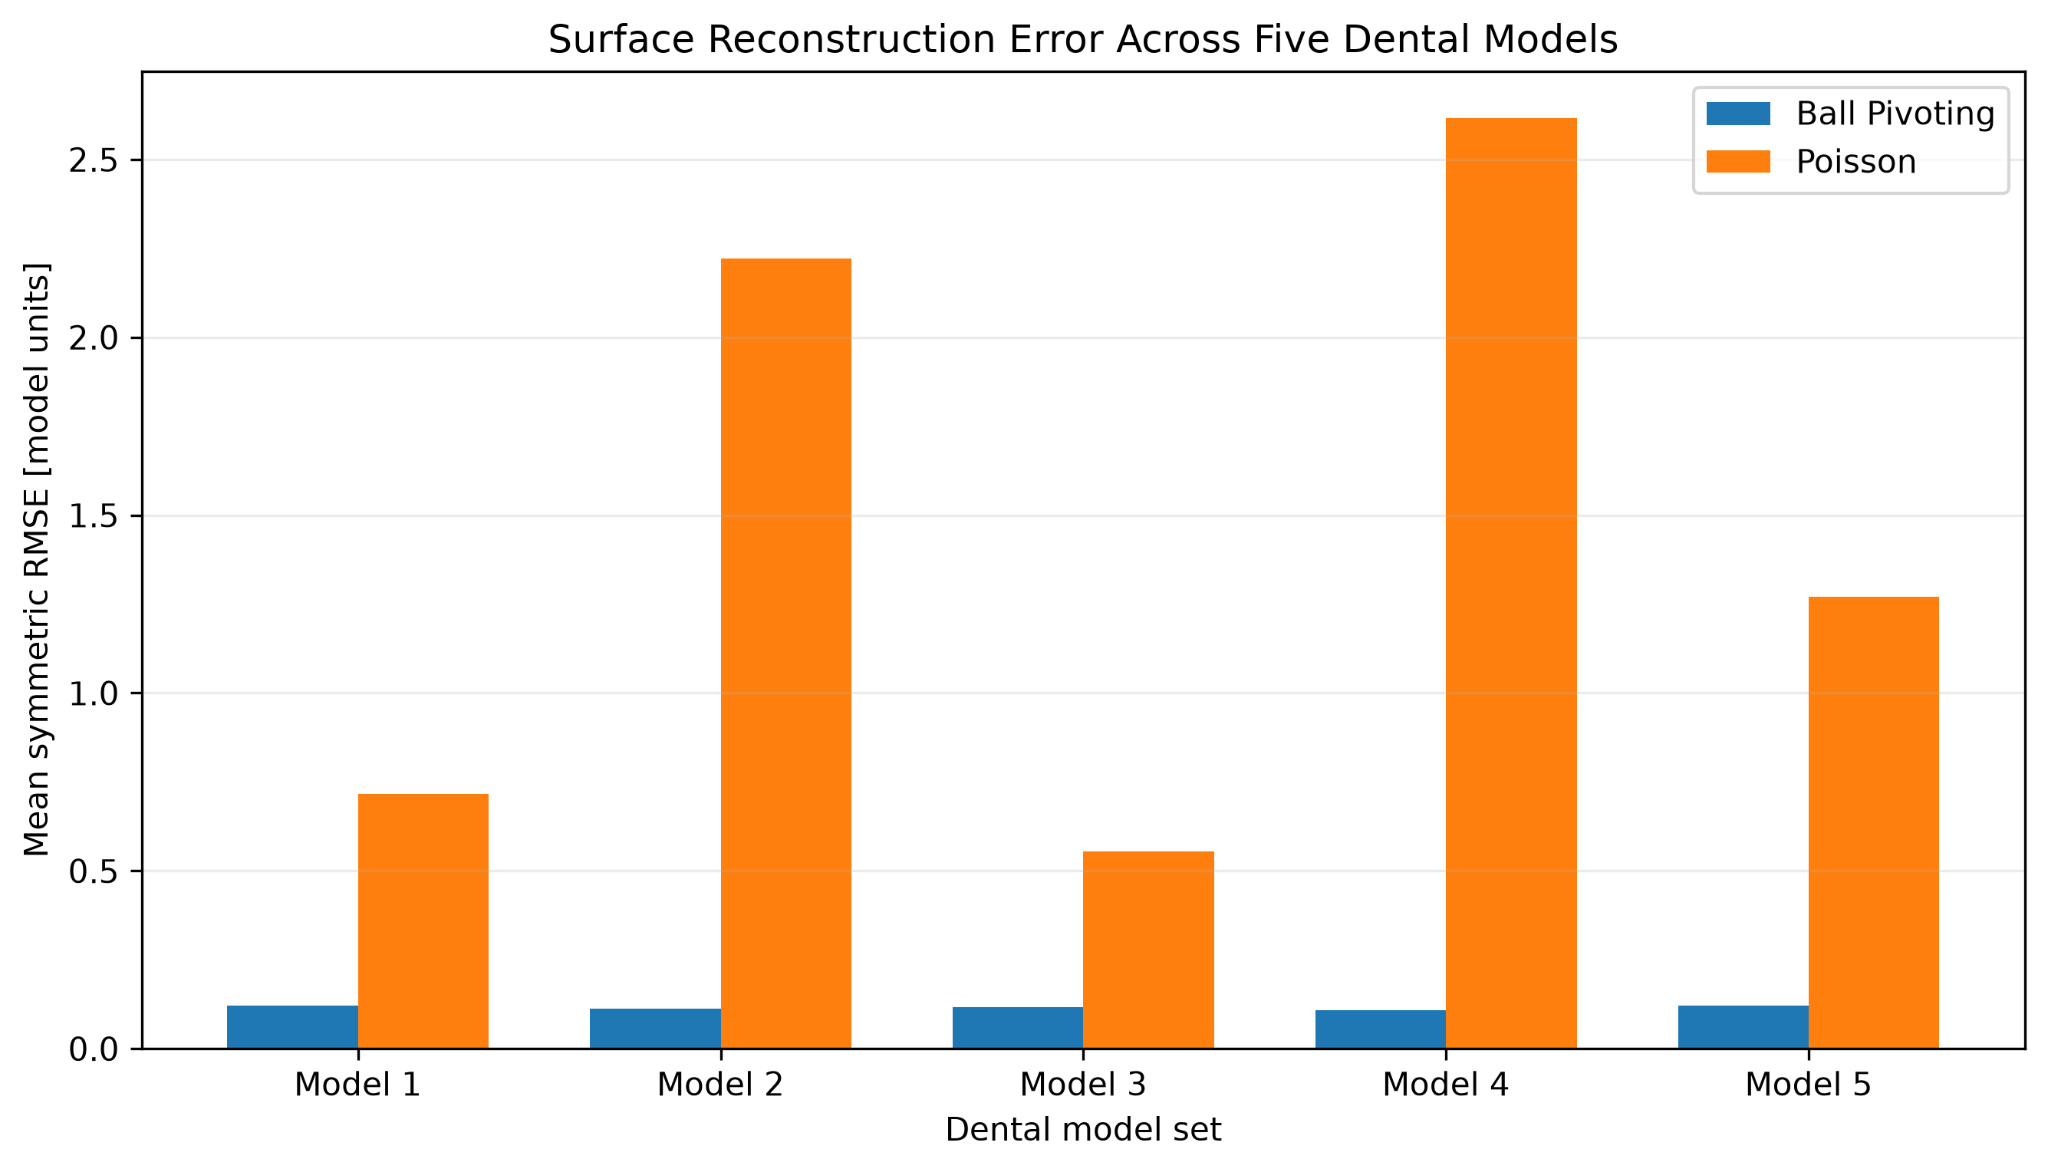
\includegraphics[width=\linewidth]{assets/marvin/model_suite/model_suite_mesh_rmse_by_model.png}
    \caption{Symmetric RMSE by model set.}
\end{subfigure}\hfill
\begin{subfigure}[t]{0.48\textwidth}
    \centering
    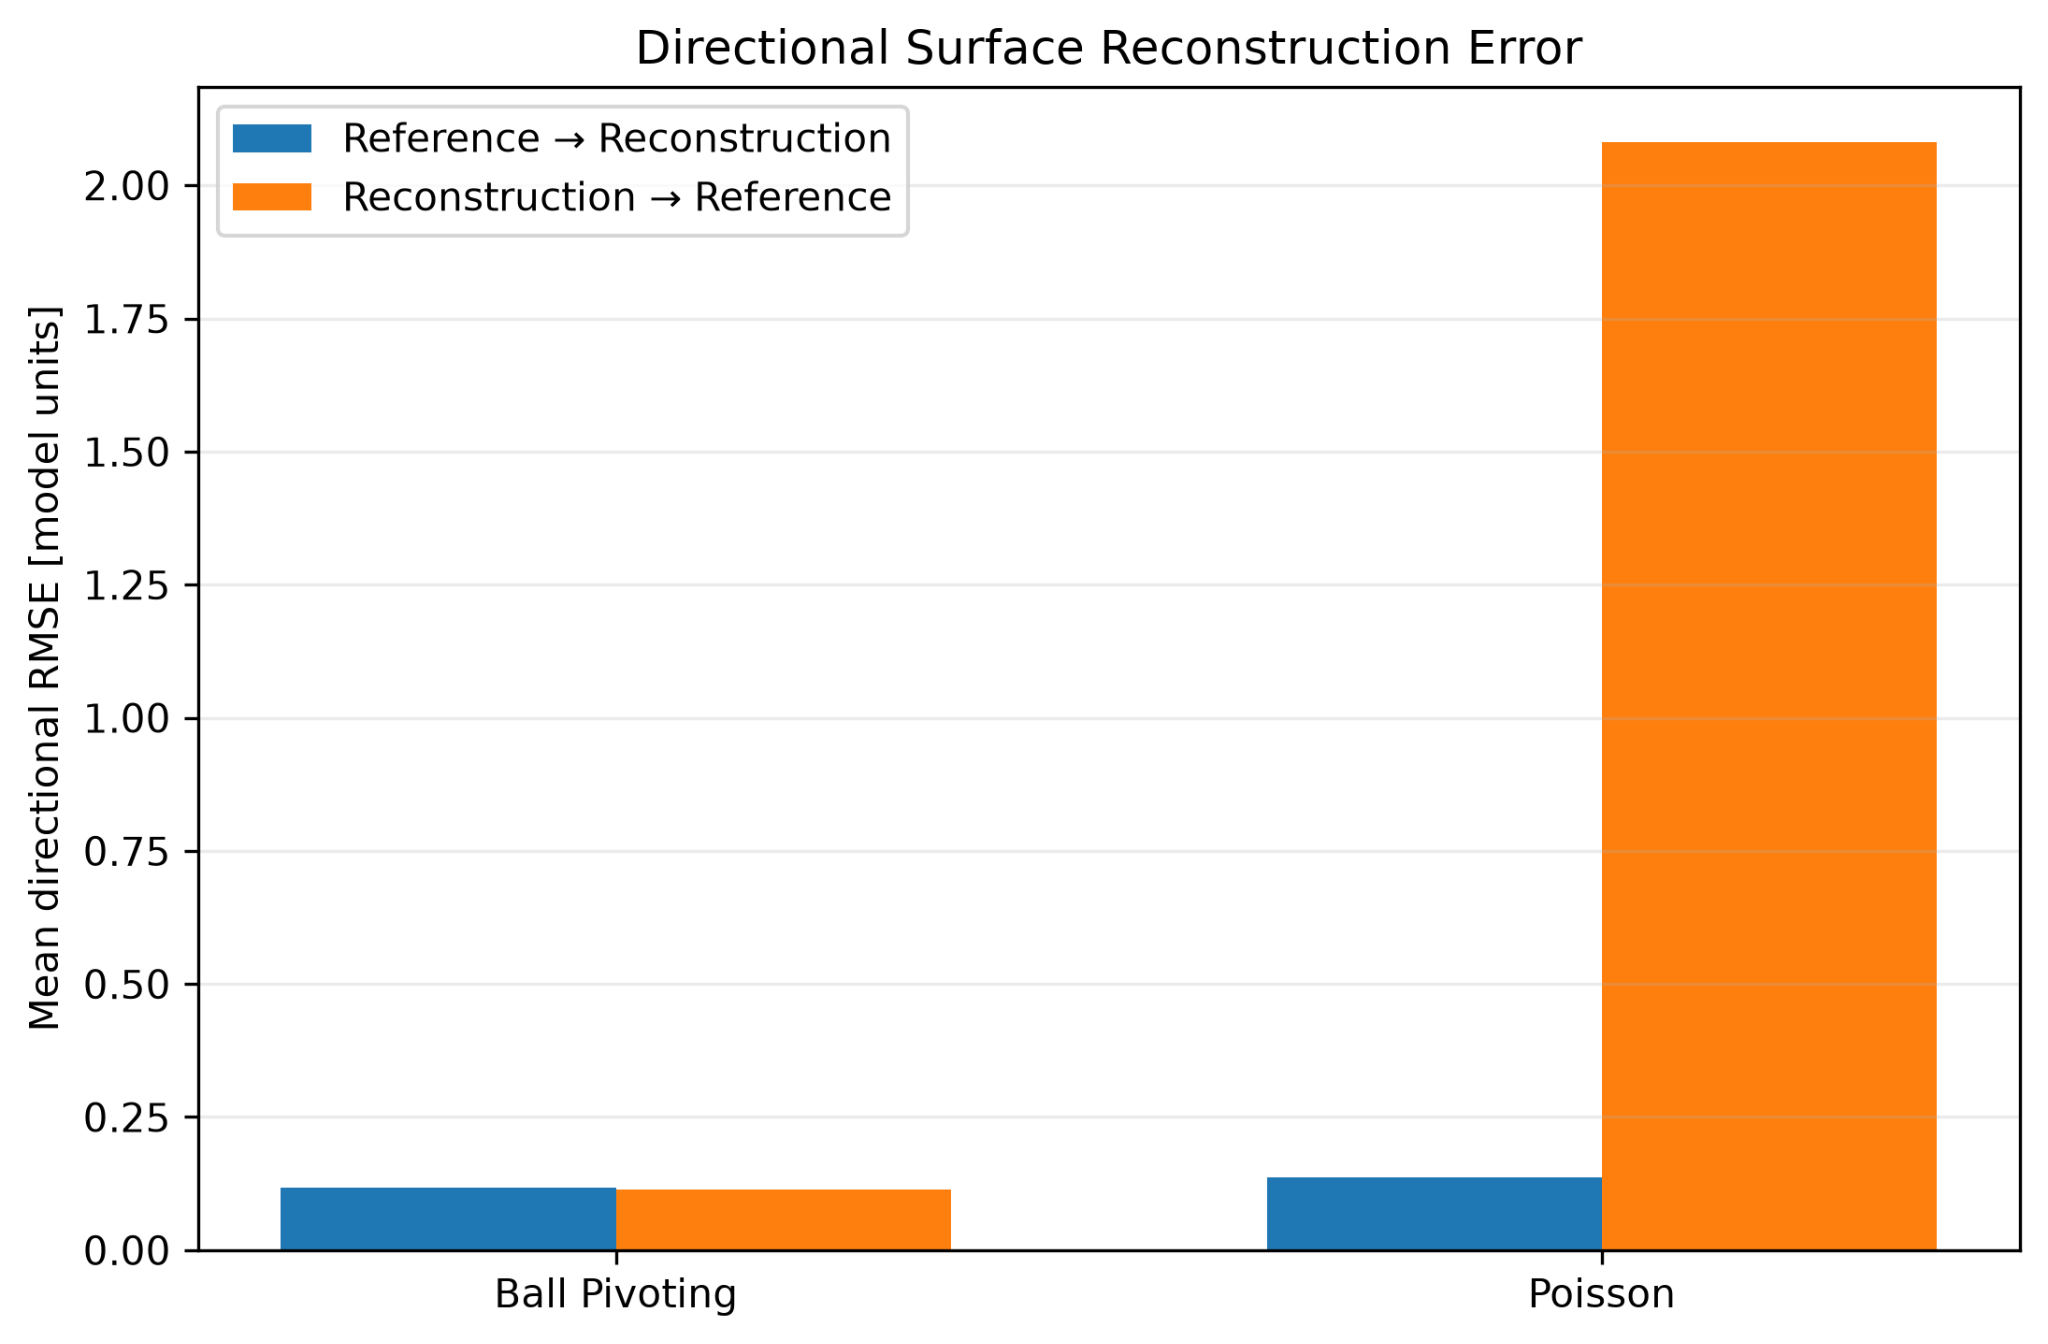
\includegraphics[width=\linewidth]{assets/marvin/model_suite/model_suite_mesh_directional_rmse.png}
    \caption{Mean directional RMSE.}
\end{subfigure}
\caption{Surface-reconstruction generalization across five dental model sets. BPA is consistently more accurate, while Poisson's dominant error occurs in the reconstruction-to-reference direction, indicating unsupported added geometry.}
\label{fig:model-suite-mesh-errors}
\end{figure*}

The directional evaluation is central to this result. Poisson covers much of the reference geometry reasonably well, with a mean reference-to-reconstruction RMSE of 0.1366 model units. In the opposite direction, however, its mean RMSE rises to 2.0807 model units, compared with only 0.1140 for BPA. The mean Poisson surface-area ratio of 1.415 indicates approximately 41.5\% more reconstructed area than the reference on average, whereas BPA remains close to the reference at 0.972. All ten Poisson meshes contain self-intersections; none of the ten BPA meshes do.

\begin{figure*}[!t]
\centering
\begin{subfigure}[t]{0.48\textwidth}
    \centering
    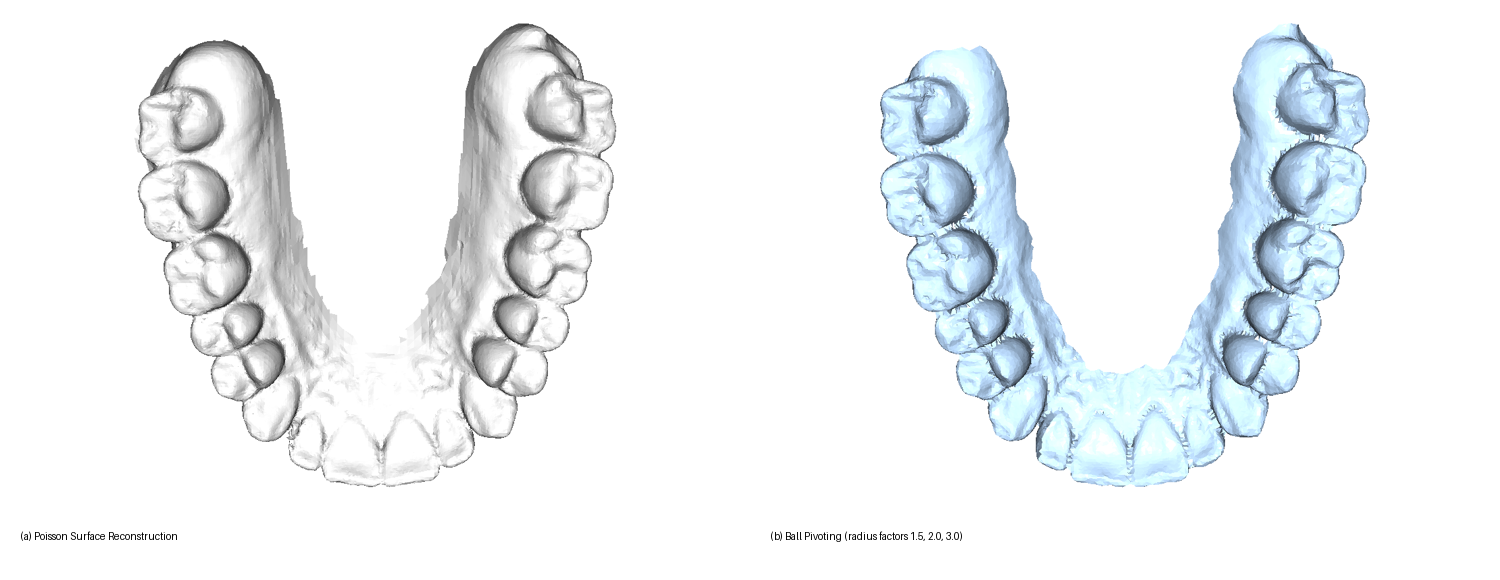
\includegraphics[width=\linewidth]{assets/marvin/realistic_poisson_vs_bpa.png}
    \caption{Representative upper-jaw comparison.}
\end{subfigure}\hfill
\begin{subfigure}[t]{0.48\textwidth}
    \centering
    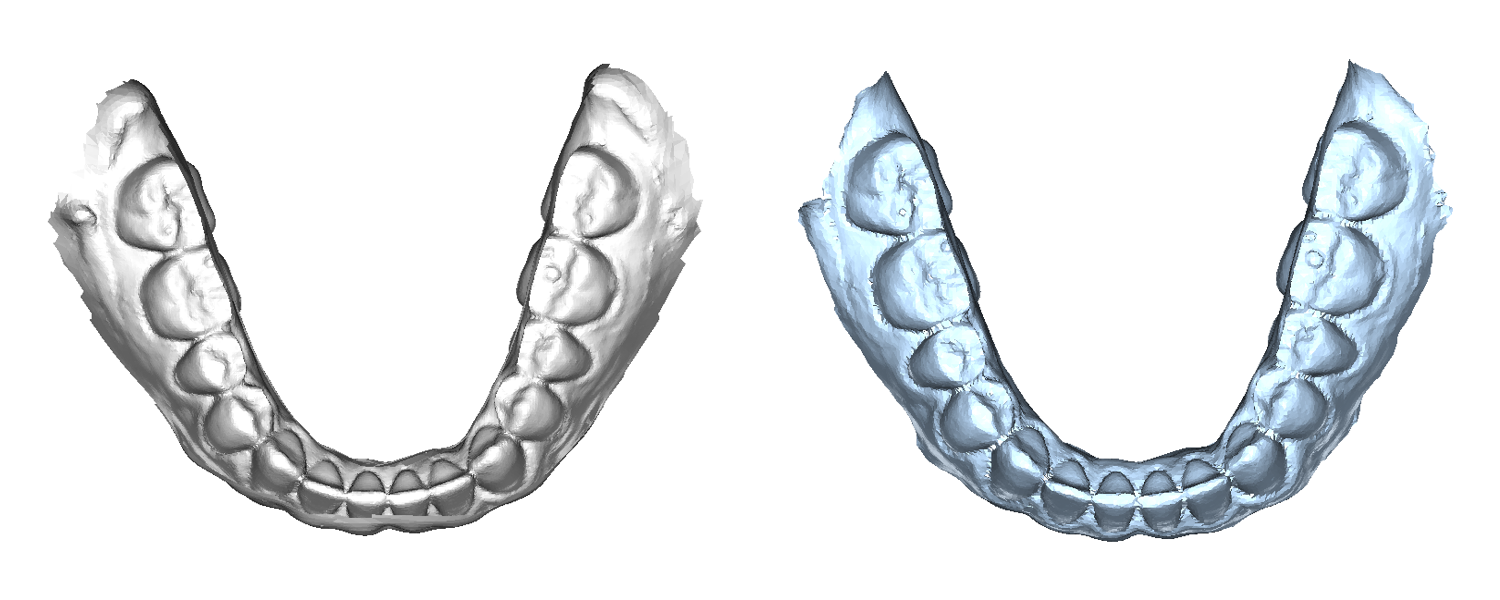
\includegraphics[width=\linewidth]{assets/marvin/lower/lower_05_poisson_vs_bpa.png}
    \caption{Representative lower-jaw comparison.}
\end{subfigure}
\caption{Representative qualitative comparison from Model~1. Poisson appears smooth and closed, but the ten-jaw quantitative evaluation shows substantially larger unsupported surface error than BPA.}
\label{fig:representative-poisson-bpa}
\end{figure*}

The final realistic reconstruction choice is therefore:
\begin{center}
\textbf{Ball Pivoting with radius factors $(1.5,2.0,3.0)$.}
\end{center}

\subsection{Discussion: Synthetic Screening versus Realistic Validation}
\label{sec:marvin-discussion}

The two-stage evaluation shows why broad synthetic screening and multi-model realistic validation serve different purposes. The synthetic generator isolates overlap, rotation, translation, and noise, which makes failure modes interpretable. The five-model suite then tests whether those conclusions survive substantial changes in actual dental geometry. The second stage both revised and strengthened the provisional choices: RANSAC replaced FGR as the final global registration method, while BPA was confirmed and its realistic radius configuration changed from A to B.

\begin{table*}[!t]
\centering
\footnotesize
\begin{tabularx}{\textwidth}{@{}lYYY@{}}
\toprule
\textbf{Decision} & \textbf{Synthetic evidence} & \textbf{Five-model realistic evidence} & \textbf{Final interpretation} \\
\midrule
Global registration & FGR offered a strong accuracy/runtime compromise in the controlled benchmark & RANSAC solved all 30 zero-noise adjacent pairs and stayed at 100\% through $\sigma=0.10$ & Select RANSAC + ICP for robustness \\
Multiway chaining & Small error in four-fragment synthetic baseline & Maximum global error across 30 non-reference poses: 0.008239 model units and $0.02266^\circ$ & Sequential four-fragment accumulation remains small \\
Surface reconstruction & BPA strongly outperformed Poisson in bidirectional error & BPA outperformed Poisson on every model set; 0/10 versus 10/10 self-intersecting meshes & Retain BPA \\
BPA radii & Configuration A minimized synthetic RMSE & B reduced boundary edges by 81.6\% versus A for only 2.4\% higher mean RMSE & Use configuration B on realistic dental geometry \\
\bottomrule
\end{tabularx}
\caption{How five-model validation revised or confirmed the provisional synthetic conclusions.}
\label{tab:synthetic-vs-realistic-discussion}
\end{table*}

A second lesson concerns metric choice. FGR often has excellent median transform errors despite catastrophic failures, so median precision alone would hide robustness problems. Likewise, Poisson can look visually smooth and has relatively few boundary edges, yet its reconstruction-to-reference error and inflated surface area reveal unsupported geometry. The final decisions therefore combine transform error, success rate, bidirectional surface distance, boundary structure, connected components, surface-area ratio, and self-intersection tests rather than relying on a single metric.

\subsection{Reproducibility and Integration into the Shared Pipeline}
\label{sec:marvin-reproducibility}

All experiments are deterministic where possible. The synthetic stress tests use 10 repetitions per condition with controlled dataset-seed ranges and reproducible algorithm seeds; the same repetition index is reused across values within a stress-test series so that the intended parameter change dominates the comparison. Open3D seed 42 is used for surface sampling. The five-model zero-noise benchmark assigns deterministic algorithm seeds to every model/jaw/pair combination. In the noise experiment, deterministic per-model, per-jaw, per-level, and per-repetition seeds generate the noisy clouds, and every algorithm receives the same perturbed geometry. Intermediate outputs are stored as PLY meshes/point clouds and CSV or NumPy files containing metrics and poses.

The module boundaries also define the hand-off to the surrounding DentaVision project. The image-acquisition and 3-D reconstruction stage provides point-cloud fragments. The present registration stage aligns these fragments and exports a merged point cloud. Surface reconstruction then produces an explicit mesh suitable for downstream visualization or later processing. Generated test fragments and intermediate outputs can be reproduced from the source STL models and are therefore not required to be versioned in the shared repository.


For the final repository organization, reusable implementation code remains under \texttt{src/registration3d}, while executable studies are grouped under a top-level \texttt{experiments/} directory. Report-figure generation and diagnostic utilities are kept separately in \texttt{visualization/} and \texttt{diagnostics/}. Historical single-model experiment drivers are archived rather than mixed with the final five-model study. This organization keeps the core package importable while making the experimental provenance of the reported numbers explicit. The principal five-model drivers are the pairwise benchmark, noise benchmark, sequential multiway benchmark, BPA parameter study, and BPA-versus-Poisson mesh validation.


\begin{table}[!t]
\centering
\scriptsize
\setlength{\tabcolsep}{3pt}
\begin{tabularx}{\columnwidth}{@{}lY@{}}
\toprule
\textbf{Experiment driver} & \textbf{Purpose} \\
\midrule
\texttt{realistic\_model\_suite\_pairwise\_benchmark.py} & Five-algorithm comparison on 30 adjacent fragment pairs \\
\texttt{realistic\_model\_suite\_noise\_benchmark.py} & Shared-noise robustness evaluation over 2,400 registrations \\
\texttt{realistic\_model\_suite\_multiway\_ransac.py} & Sequential four-fragment RANSAC multiway evaluation \\
\texttt{realistic\_model\_suite\_bpa\_parameter\_study.py} & BPA radius trade-off across ten jaws \\
\texttt{realistic\_model\_suite\_mesh\_validation.py} & Final BPA-versus-Poisson surface comparison \\
\bottomrule
\end{tabularx}
\caption{Principal final experiment drivers after repository cleanup. All are executed from the project root through the Poetry environment.}
\label{tab:experiment-drivers}
\end{table}

\begin{table}[!t]
\centering
\footnotesize
\begin{tabularx}{\columnwidth}{@{}lY@{}}
\toprule
\textbf{Artifact} & \textbf{Role in pipeline} \\
\midrule
Fragment PLY files & Pairwise and multiway registration input \\
Estimated pose arrays & Reproducible multiway transformation state \\
Merged point cloud & Interface between registration and mesh reconstruction \\
Evaluation CSV/JSON & Quantitative experiment results \\
Final PLY mesh & Indexed geometry for processing and visualization \\
Final STL mesh & Interoperable triangular surface export \\
\bottomrule
\end{tabularx}
\caption{Principal artifacts exchanged or exported by the registration/model-construction stage.}
\label{tab:pipeline-artifacts}
\end{table}

\subsection{Final Method Selection and Limitations}
\label{sec:marvin-final-selection}

The final method selection differs from the provisional synthetic choice because the realistic validation exposed failure modes that were not sufficiently represented by the first synthetic benchmark.

\begin{table}[H]
\centering
\scriptsize
\setlength{\tabcolsep}{2.5pt}
\begin{tabularx}{\columnwidth}{@{}lYY@{}}
\toprule
\textbf{Stage} & \textbf{Final choice} & \textbf{Key evidence} \\
\midrule
Pairwise & \textbf{FPFH + RANSAC + P2Plane ICP} & 30/30 zero-noise successes; strongest noise robustness \\
Multiway & \textbf{Sequential four-fragment chaining} & Explicit pairwise-error accumulation without loop-closure correction \\
Surface & \textbf{Ball Pivoting} & Lower bidirectional error; 0/10 self-intersecting meshes \\
BPA radii & \textbf{$(1.5,2.0,3.0)$} & 81.6\% fewer boundary edges than A for 2.4\% higher mean RMSE \\
Simplification & \textbf{$\approx$30k triangles} & 25.04\% triangle reduction for 0.171\% RMSE increase in synthetic study \\
\bottomrule
\end{tabularx}
\caption{Final design decisions after synthetic screening and five-model realistic validation.}
\label{tab:final-selection}
\end{table}

\subsubsection{Threats to Validity}

\paragraph{Internal validity.}
The experiments were designed to make algorithmic differences dominate over incidental randomness. All methods within one noisy trial receive exactly the same perturbed point clouds, dataset and algorithm seeds are deterministic, and pairwise transformations can be evaluated against exact virtual ground truth. Nevertheless, stochastic global registration can still exhibit seed-dependent outcomes. The reported benchmark therefore characterizes the implemented configuration and seed-controlled protocol rather than every possible random realization. The Wilson intervals shown for RANSAC visualize finite-sample uncertainty only; the three nonzero-noise repetitions share the same 30 base fragment pairs and are not treated as 90 independent dental geometries.

\paragraph{Construct validity.}
Correctness is operationalized by transform error when ground truth is available, using thresholds of one model unit and one degree in the realistic registration study. These thresholds are deliberately more informative than fitness or inlier RMSE alone, because repetitive dental surfaces can support plausible but incorrect correspondence sets. Surface quality is likewise assessed bidirectionally instead of relying only on appearance or watertightness. However, the mesh-distance evaluation is sampling based and therefore approximates, rather than exactly computes, point-to-triangle surface distance. In addition, STL does not encode physical units, so absolute distances are reported in model units and should not be interpreted as millimeters without verified source metadata.

\paragraph{External validity.}
The five realistic model sets are STL surfaces that are sampled and fragmented in software; they are substantially more diverse than the synthetic dental-like generator but are not actual intraoral scanner captures. Real acquisitions may contain occlusions, outliers, strongly nonuniform point density, reflections, motion artifacts, and scanner-specific systematic error. The added perturbation is isotropic Gaussian positional noise rather than a calibrated sensor-noise model. Furthermore, the ten jaws have intentionally similar overall scale and do not systematically cover severe malocclusions, missing teeth, restorations, pathological anatomy, or deliberately varied acquisition conditions. Generalization to those clinically relevant geometry classes therefore remains untested. Finally, the realistic multiway experiment evaluates four-fragment sequential chaining without loop closures; substantially longer acquisition trajectories may require pose-graph optimization and explicit loop-consistency checks.

\FloatBarrier
\subsection{Conclusion}
\label{sec:marvin-conclusion}

A complete registration and model-construction pipeline was implemented and evaluated from multiple dental point-cloud fragments to reconstructed triangular surfaces. Five pairwise registration algorithms were first compared under controlled synthetic changes in overlap, rotation, translation, and noise. The synthetic benchmark initially favored FPFH + FGR + Point-to-Plane ICP, but the subsequent five-model validation exposed catastrophic FGR outliers and changed the final selection to FPFH + RANSAC + Point-to-Plane ICP.

Across five distinct dental model sets comprising ten jaw meshes and 30 adjacent zero-noise fragment pairs, the selected RANSAC pipeline achieved 30/30 successful registrations with mean translation and rotation errors of 0.001921 model units and $0.00948^\circ$. Under added Gaussian positional noise it maintained 100\% observed success through $\sigma=0.10$ and achieved 84.44\% at $\sigma=0.20$. Sequential four-fragment multiway registration across all ten jaws yielded a maximum global pose error of only 0.008239 model units and $0.02266^\circ$.

For surface reconstruction, BPA configuration B $(1.5,2.0,3.0)$ provided the best realistic trade-off between geometric fidelity and boundary closure. Across all ten jaw meshes, BPA achieved a mean symmetric RMSE of 0.115989 compared with 1.475913 for Poisson. Poisson's mean reconstruction-to-reference RMSE reached 2.080730 and its mean area ratio 1.414758, indicating substantial unsupported geometry; all ten Poisson meshes contained self-intersections, whereas none of the BPA meshes did.

The main outcome is therefore not only a final algorithm choice but a reproducible selection strategy: controlled synthetic experiments expose specific failure modes, while multi-model realistic geometry determines which methods generalize sufficiently well to be carried forward into the DentaVision pipeline.
